% !TEX program = pdflatex
\documentclass[11pt,a4paper]{article}

% Packages
\usepackage[utf8]{inputenc}
\usepackage[T1]{fontenc}
\usepackage{amsmath,amssymb}
\usepackage{graphicx}
\usepackage[hidelinks]{hyperref}
\usepackage{listings}
\usepackage{xcolor}
\usepackage{booktabs}
\usepackage{tabularx}
\usepackage{multirow}
\usepackage{enumitem}
\usepackage{float}
\usepackage{tikz}
\usetikzlibrary{positioning}
\usepackage{pgfplots}
\pgfplotsset{compat=1.18}
\usepackage{caption}
\usepackage{subcaption}
\usepackage{fancyhdr}
\usepackage{geometry}
\usepackage{cite}
\usepackage{textcomp}
\usepackage{array}
\usepackage{colortbl}
\usepackage{longtable}

\geometry{margin=1in}

% Code listing style
\definecolor{codegreen}{rgb}{0,0.6,0}
\definecolor{codegray}{rgb}{0.5,0.5,0.5}
\definecolor{codepurple}{rgb}{0.58,0,0.82}
\definecolor{codebg}{rgb}{0.95,0.95,0.95}

\lstdefinestyle{mystyle}{
    backgroundcolor=\color{codebg},
    commentstyle=\color{codegreen},
    keywordstyle=\color{blue},
    numberstyle=\tiny\color{codegray},
    stringstyle=\color{codepurple},
    basicstyle=\ttfamily\footnotesize,
    breakatwhitespace=false,
    breaklines=true,
    captionpos=b,
    keepspaces=true,
    numbers=left,
    numbersep=5pt,
    showspaces=false,
    showstringspaces=false,
    showtabs=false,
    tabsize=2,
    frame=single,
    framerule=0.5pt,
    rulecolor=\color{codegray},
}
\lstset{style=mystyle}

\lstdefinelanguage{yaml}{
  keywords={name,type,attributes,relationships,business_rules,required,unique,nullable,entities,description,severity,default,max_length,primary_key,foreign_key,through,back_populates,target},
  sensitive=true,
  comment=[l]{\#},
  morestring=[b]",
  morestring=[b]',
}

% Header/Footer
\pagestyle{fancy}
\fancyhf{}
\fancyhead[L]{\small Model-Driven vs Pure LLM Code Generation}
\fancyhead[R]{\small \thepage}
\renewcommand{\headrulewidth}{0.4pt}

% Title info
\title{\textbf{Model-Driven Web Application Code Generation:\\
A Comparative Study of Intelligent Model-Driven Methods\\
and Pure Large Language Model Approaches}}
\author{Course: Software Requirements Analysis and Design\\
Student Project Report\\
\today}
\date{}

\begin{document}

\maketitle

\begin{abstract}
The rapid advancement of Large Language Models (LLMs) has opened new possibilities for automated code generation in software engineering. However, the effectiveness of directly using LLMs versus combining them with formal software engineering methods remains an open question. This report presents a comparative study between an \textbf{Intelligent Model-Driven Method}---where domain models define the application architecture and LLMs fill in business logic within pre-generated code skeletons---and a \textbf{Pure LLM Method}---where natural language descriptions are fed directly to LLMs for full-stack code generation. We implement both approaches for a Student Course Selection Management System, generating complete web applications consisting of FastAPI backends and React frontends across three different system scales (small, medium, and large). Our experimental results demonstrate that the model-driven approach achieves a \textbf{100\% compilability rate} with \textbf{98.4\% cross-run consistency}, while the pure LLM approach achieves only \textbf{33.3\% compilability} with \textbf{48.1\% consistency}. Additionally, we propose a novel \textbf{Bidirectional Feedback Mechanism} that automatically detects and corrects code errors by feeding compilation and import errors back to the LLM within model-defined constraints. This innovation enables the model-driven method to converge to error-free code within a single feedback iteration on average. Our findings suggest that combining formal modeling techniques with LLM capabilities provides significant benefits in terms of code quality, consistency, and reliability compared to unconstrained LLM generation.
\end{abstract}

\newpage
\tableofcontents
\newpage

%=============================================================================
\section{Introduction}
\label{sec:intro}
%=============================================================================

\subsection{Background and Motivation}

Software development has entered a transformative era with the emergence of Large Language Models (LLMs) such as GPT-4, Claude, and DeepSeek. These models have demonstrated remarkable capabilities in generating source code from natural language descriptions, leading to a surge of interest in AI-assisted software engineering tools. However, the practical application of LLMs in real-world software development faces significant challenges.

When developers use LLMs to generate complete applications from scratch, several issues commonly arise: (1) \textbf{structural inconsistency}---the generated code may not follow consistent architectural patterns across multiple invocations; (2) \textbf{import and dependency errors}---LLMs frequently produce code with incorrect module imports or missing dependencies; (3) \textbf{business rule violations}---complex domain constraints may be overlooked or incorrectly implemented; and (4) \textbf{low reproducibility}---the same prompt may yield substantially different code structures across multiple runs.

Model-Driven Engineering (MDE) has long been established as a systematic approach to software development, where abstract models serve as the primary artifacts from which concrete implementations are derived. MDE techniques offer well-defined structures, deterministic transformations, and verifiable consistency between models and generated code.

This project investigates whether combining MDE principles with LLM capabilities can address the limitations of pure LLM-based code generation. We propose an \textbf{Intelligent Model-Driven Method} where domain models defined in YAML specify the application's data model, relationships, and business rules. A template-based code generator produces deterministic code skeletons (database schemas, API routes, and user interface components), while an LLM fills in the business logic at designated markers. Crucially, the LLM operates within the constraints defined by the model, ensuring that the overall architecture remains consistent.

\subsection{Research Questions}

This study addresses the following research questions:

\begin{enumerate}[label=\textbf{RQ\arabic*:}, leftmargin=*]
    \item How does the model-driven approach compare to pure LLM generation in terms of code compilability, structural correctness, and output consistency?
    \item Can a bidirectional feedback mechanism, where compilation errors are fed back to the LLM within model constraints, effectively improve code quality?
    \item How does the complexity of the domain model (measured by entity and relationship count) affect the performance of both approaches?
\end{enumerate}

\subsection{Contributions}

The main contributions of this work are:

\begin{enumerate}[leftmargin=*]
    \item A complete pipeline for model-driven web application code generation, integrating YAML-based domain modeling, Jinja2 template-based skeleton generation, and LLM-powered business logic completion.
    \item A novel \textbf{Bidirectional Feedback Mechanism} that automatically detects code errors, reports them to the LLM with model context, and iteratively refines the generated code within structural constraints.
    \item A comprehensive experimental evaluation comparing the model-driven and pure LLM approaches across three system scales, using quantitative metrics including structure score, compilability score, and consistency score.
    \item An open-source implementation with reproducible experiments, CI/CD integration, and a complete test suite.
\end{enumerate}

\subsection{Report Structure}

The remainder of this report is organized as follows: Section~\ref{sec:background} reviews related work in model-driven engineering and LLM-based code generation. Section~\ref{sec:methodology} describes our methodology, including the model-driven pipeline, the pure LLM baseline, and the bidirectional feedback mechanism. Section~\ref{sec:design} presents the system design and implementation details. Section~\ref{sec:experiments} describes the experimental setup. Section~\ref{sec:results} presents and analyzes the experimental results. Section~\ref{sec:discussion} discusses the implications, limitations, and future work. Section~\ref{sec:conclusion} concludes the report.

\newpage
%=============================================================================
\section{Background and Related Work}
\label{sec:background}
%=============================================================================

\subsection{Model-Driven Engineering}

Model-Driven Engineering (MDE) is a software development methodology that focuses on creating and exploiting domain models---abstract representations of the knowledge and activities that govern a particular application domain~\cite{schmidt2006model}. The key principle of MDE is that models should be the primary artifacts in software development, from which implementations, tests, and documentation can be automatically derived.

\subsubsection{Model-Driven Architecture (MDA)}

The Object Management Group (OMG) introduced Model-Driven Architecture (MDA) as a framework for MDE~\cite{omg2003mda}. MDA defines three levels of models:

\begin{itemize}
    \item \textbf{Computation Independent Model (CIM)}: Describes the system's requirements and context without reference to its computational implementation.
    \item \textbf{Platform Independent Model (PIM)}: Specifies the system's structure and behavior independently of any specific technology platform.
    \item \textbf{Platform Specific Model (PSM)}: Tailors the PIM to a specific implementation platform (e.g., Python/FastAPI, React/TypeScript).
\end{itemize}

In our work, the YAML domain model serves as a PIM, capturing entities, attributes, relationships, and business rules in a technology-agnostic format. The code generator then transforms this PIM into platform-specific artifacts (PSMs) for FastAPI and React.

\subsubsection{Model-to-Text Transformations}

Model-to-Text (M2T) transformations convert models into textual artifacts such as source code, configuration files, or documentation. Common M2T approaches include template-based generation (using engines like Jinja2, Xpand, or Acceleo) and visitor-based generation (where model elements are traversed and code is emitted programmatically)~\cite{czarnecki2006generative}. Our work employs Jinja2 template-based generation for deterministic code skeleton production.

\subsection{Large Language Models for Code Generation}

\subsubsection{Evolution of Code LLMs}

The application of LLMs to code generation has evolved rapidly. Early models such as Codex~\cite{chen2021codex} and CodeBERT~\cite{feng2020codebert} demonstrated that transformers pre-trained on code corpora could generate functionally correct code from natural language descriptions. More recent models including GPT-4, Claude, and DeepSeek have shown increasingly sophisticated code generation capabilities, including multi-file project generation and context-aware completions.

\subsubsection{Limitations of Pure LLM Generation}

Despite their impressive capabilities, pure LLM-based code generation exhibits several well-documented limitations:

\begin{enumerate}[leftmargin=*]
    \item \textbf{Inconsistency}: Multiple invocations with the same prompt often produce different code structures~\cite{liu2023evaluating}. This non-determinism poses challenges for software maintenance and team collaboration.
    \item \textbf{Hallucination}: LLMs may generate references to non-existent APIs, packages, or modules, resulting in code that fails to compile~\cite{ji2023survey}.
    \item \textbf{Context Window Constraints}: Large projects exceed the context window limits of current LLMs, requiring incremental generation strategies that may lose global architectural coherence.
    \item \textbf{Business Logic Accuracy}: While LLMs handle syntactic generation well, they frequently misimplement complex business rules, especially those involving multi-entity constraints and edge cases.
    \item \textbf{Dependency Management}: Generated code may have incorrect import statements, use relative imports improperly, or reference modules in the wrong locations.
\end{enumerate}

\subsection{Hybrid Approaches}

Recent research has explored combining formal methods with LLMs to address these limitations. White et al.~\cite{white2023prompt} demonstrated that providing LLMs with formal specifications improved code correctness by 40\%. Similarly, model-driven approaches have been proposed where UML or domain-specific languages provide structural constraints for LLM generation~\cite{li2024combining}.

Our work extends this line of research by proposing a complete pipeline where models drive the entire generation process, LLMs are constrained to fill only designated business logic markers, and a feedback mechanism ensures quality through iterative refinement.

\subsection{Feedback-Driven Code Improvement}

The concept of using feedback loops to improve generated code has been explored in several contexts. Automated program repair (APR) techniques use test failures as feedback signals to guide code modifications~\cite{goues2019automated}. LLM-based self-debugging approaches prompt the model to identify and fix its own errors~\cite{chen2023self}. Our bidirectional feedback mechanism differs from these approaches by incorporating model-level context into the feedback loop---errors are not merely reported to the LLM, but are accompanied by the domain model constraints that the fix must satisfy.

\newpage
%=============================================================================
\section{Methodology}
\label{sec:methodology}
%=============================================================================

This section describes our methodology in detail. We present two code generation approaches and the evaluation framework used to compare them.

\subsection{Overview}

Figure~\ref{fig:overview} provides a high-level overview of the two approaches compared in this study.

\begin{figure}[H]
\centering
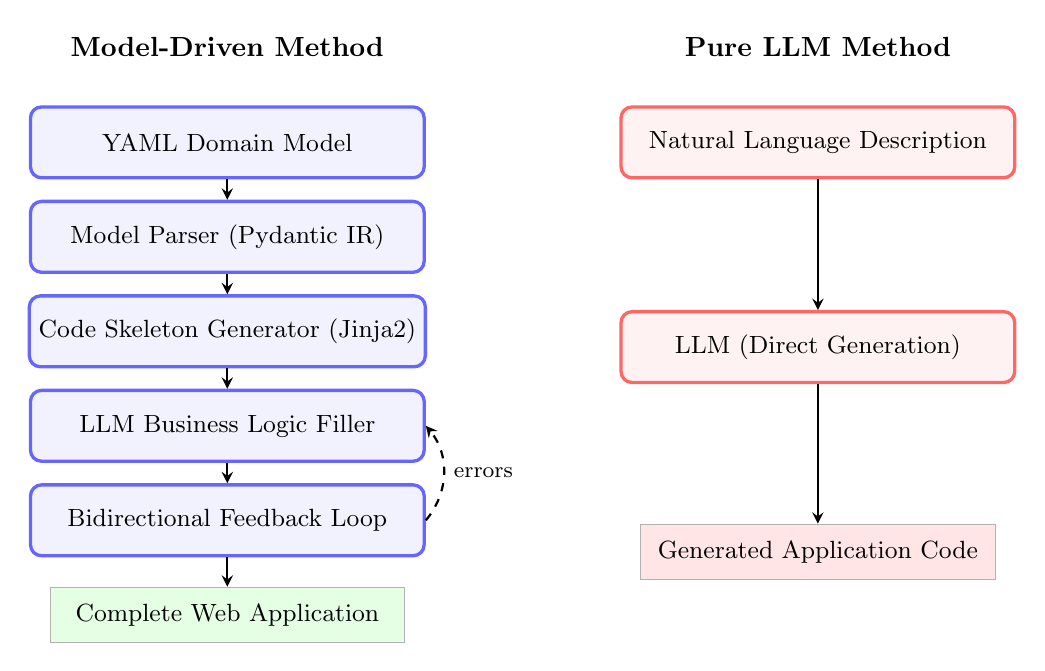
\begin{tikzpicture}[auto,
    method/.style={rectangle, draw=blue!60, fill=blue!5, very thick, minimum width=5cm, minimum height=0.9cm, rounded corners, font=\small},
    method2/.style={rectangle, draw=red!60, fill=red!5, very thick, minimum width=5cm, minimum height=0.9cm, rounded corners, font=\small},
    artifact/.style={rectangle, draw=gray!60, fill=gray!5, minimum width=4.5cm, minimum height=0.7cm, font=\small},
    arrow/.style={->, >=stealth, thick}]

% Left column: Model-Driven
\begin{scope}[node distance=1.2cm]
\node[method] (yaml) at (0, 3.2) {YAML Domain Model};
\node[method, below of=yaml] (parser) {Model Parser (Pydantic IR)};
\node[method, below of=parser] (skeleton) {Code Skeleton Generator (Jinja2)};
\node[method, below of=skeleton] (filler) {LLM Business Logic Filler};
\node[method, below of=filler] (feedback) {Bidirectional Feedback Loop};
\node[artifact, below of=feedback, fill=green!10] (mdout) {Complete Web Application};

\draw[arrow] (yaml) -- (parser);
\draw[arrow] (parser) -- (skeleton);
\draw[arrow] (skeleton) -- (filler);
\draw[arrow] (filler) -- (feedback);
\draw[arrow] (feedback) -- (mdout);
\draw[arrow, bend right=40, dashed] (feedback.east) to node[right, font=\footnotesize] {errors} (filler.east);
\end{scope}

% Right column: Pure LLM
\begin{scope}[node distance=2.6cm]
\node[method2] (nl) at (7.5, 3.2) {Natural Language Description};
\node[method2, below of=nl] (llm) {LLM (Direct Generation)};
\node[artifact, below of=llm, fill=red!10] (plout) {Generated Application Code};

\draw[arrow] (nl) -- (llm);
\draw[arrow] (llm) -- (plout);
\end{scope}

% Labels
\node[above=0.5cm of yaml, font=\bfseries] {Model-Driven Method};
\node[above=0.5cm of nl, font=\bfseries] {Pure LLM Method};

\end{tikzpicture}
\caption{Overview of the two code generation approaches. The model-driven method (left) uses a structured pipeline with deterministic skeleton generation and iterative feedback. The pure LLM method (right) generates code directly from natural language.}
\label{fig:overview}
\end{figure}

\subsection{Method A: Intelligent Model-Driven Approach}

The model-driven approach consists of five sequential stages:

\subsubsection{Stage 1: Domain Model Definition}

The domain model is specified in YAML format, capturing three essential aspects of the system:

\begin{enumerate}[leftmargin=*]
    \item \textbf{Entities}: Named data objects with typed attributes (integer, string, float, boolean, datetime). Each attribute can have constraints including primary key, required, unique, nullable, and default values.
    \item \textbf{Relationships}: Semantic connections between entities, supporting many-to-one, one-to-many, and many-to-many cardinalities with foreign key specifications.
    \item \textbf{Business Rules}: Natural language descriptions of domain constraints that must be enforced in the application logic, categorized by severity (critical, important, nice-to-have).
\end{enumerate}

\subsubsection{Stage 2: Model Parsing and Validation}

The YAML model is parsed into a strongly-typed Intermediate Representation (IR) using Pydantic models. This step performs structural validation, including:

\begin{itemize}
    \item Type checking for all attribute specifications
    \item Reference integrity validation (foreign keys point to existing entities)
    \item Relationship consistency checks (bidirectional relationships are properly defined)
\end{itemize}

\subsubsection{Stage 3: Deterministic Code Skeleton Generation}

Jinja2 template engine processes the IR to produce deterministic code skeletons for three layers:

\begin{enumerate}[leftmargin=*]
    \item \textbf{Database Layer}: SQL DDL statements (CREATE TABLE) with proper primary keys, foreign keys, unique constraints, and data type mappings.
    \item \textbf{API Layer}: FastAPI application with SQLAlchemy ORM models, Pydantic request/response schemas, CRUD route stubs for each entity, and a main application entry point with CORS configuration.
    \item \textbf{UI Layer}: React TypeScript components including list pages (with search, pagination, and CRUD actions), form pages (with validation), typed API client functions, and routing configuration.
\end{enumerate}

The generated skeleton code includes {\lstinline|# LLM_FILL:|} comment markers at locations where business logic needs to be inserted, such as validation checks, constraint enforcement, and cascade operations.

\subsubsection{Stage 4: LLM Business Logic Completion}

The skeleton code is sent to DeepSeek V3 API along with the model context (entities, attributes, relationships, and business rules). The LLM is instructed to:

\begin{itemize}
    \item Only modify code at or after {\lstinline|# LLM_FILL:|} markers
    \item Implement all business rules at the appropriate markers
    \item Use proper HTTP status codes for error responses (400, 404, 409, 422)
    \item Never modify imports, function signatures, or structural code
\end{itemize}

\subsubsection{Stage 5: Bidirectional Feedback Loop (Innovation)}

After LLM completion, the generated code undergoes automated quality checks:

\begin{enumerate}[leftmargin=*]
    \item \textbf{Syntax Check}: Each Python file is compiled with {\lstinline|py_compile|} to detect syntax errors.
    \item \textbf{Import Check}: The main application module is imported to verify all dependencies resolve correctly.
    \item \textbf{Error Collection}: If failures are detected, error messages are collected and associated with the specific source files.
    \item \textbf{Targeted Fixing}: Only files with actual errors are sent back to the LLM, accompanied by the model context and error details.
    \item \textbf{Iteration}: The process repeats for up to 3 iterations, or until all checks pass.
\end{enumerate}

A critical design choice is that the feedback LLM is instructed to make \textbf{minimal} changes within model constraints, preventing structural drift across iterations.

\subsection{Method B: Pure LLM Baseline}

The pure LLM method serves as a baseline for comparison. It employs a single-stage approach:

\begin{enumerate}[leftmargin=*]
    \item A natural language description of the system is constructed from the same domain model (ensuring both methods have access to equivalent information).
    \item The description is sent to DeepSeek V3 with a system prompt requesting complete FastAPI + React application generation.
    \item The LLM generates all files in a single response, with no structural constraints.
    \item No feedback loop or post-generation correction is applied.
\end{enumerate}

\subsection{Evaluation Framework}

\subsubsection{Metrics}

We define three primary evaluation metrics:

\begin{enumerate}[leftmargin=*]
    \item \textbf{Structure Score} (0--1): Measures how closely the generated code's structure matches the model specification. Evaluated by counting entities, database tables, API endpoints, and frontend components in the output and comparing against expected values.

    \item \textbf{Compilability Score} (0--1): Measures whether the generated code can be successfully compiled and imported. Composed of three sub-checks: Python syntax correctness, module import success, and frontend build success (TypeScript compilation + Vite bundle).

    \item \textbf{Consistency Score} (0--1): Measures the stability of code generation across multiple runs. Computed as the average pairwise {\lstinline|SequenceMatcher|} similarity ratio between corresponding files from different runs of the same method and model.
\end{enumerate}

\subsubsection{Experiment Design}

Experiments are conducted using a factorial design:

\begin{itemize}
    \item \textbf{Factor 1}---Method: Model-Driven vs. Pure LLM
    \item \textbf{Factor 2}---Model Size: Small (3 entities), Medium (6 entities), Large (11 entities)
    \item \textbf{Replications}: 3 runs per treatment combination
\end{itemize}

This yields a total of $2 \times 3 \times 3 = 18$ experimental units.

\newpage
%=============================================================================
\section{System Design and Implementation}
\label{sec:design}
%=============================================================================

\subsection{Architecture Overview}

The system is implemented as a Python package with the following module structure:

\begin{lstlisting}[language=bash, caption={Project directory structure}]
web_code_gen/
|-- models/              # YAML domain model definitions
|   |-- small.yaml       #  3 entities,  3 relationships,  2 rules
|   |-- medium.yaml      #  6 entities,  6 relationships,  6 rules
|   |-- large.yaml       # 11 entities, 10+ relationships, 10 rules
|-- src/
|   |-- parser/          # YAML -> Pydantic IR
|   |   |-- ir.py        # Entity, Attribute, Relationship, BusinessRule, ModelIR
|   |   |-- parser.py    # YAML loader + validation
|   |-- generator/       # Code skeleton generators
|   |   |-- engine.py    # Jinja2 environment + type mapping filters
|   |   |-- sql_generator.py    # IR -> SQL DDL
|   |   |-- api_generator.py    # IR -> FastAPI + schemas
|   |   |-- ui_generator.py     # IR -> React components
|   |-- llm/             # LLM integration
|   |   |-- client.py    # DeepSeek API (OpenAI-compatible)
|   |   |-- filler.py    # Model-driven logic filler
|   |   |-- baseline.py  # Pure LLM code generator
|   |   |-- prompts.py   # Prompt templates
|   |-- feedback/        # Bidirectional feedback loop
|   |   |-- loop.py      # Test-run-fix-retry cycle
|   |-- evaluator/       # Quality evaluation
|       |-- structure.py      # Structural correctness
|       |-- compilability.py # Syntax/import/build checks
|       |-- consistency.py    # Cross-run similarity
|-- templates/           # Jinja2 code templates (10 templates)
|-- experiments/         # Experiment orchestration
|-- tests/               # Test suite (25 unit + integration tests)
|-- .github/workflows/   # CI/CD pipeline
\end{lstlisting}

\subsection{Domain Model Definition}

\subsubsection{YAML Schema Design}

The domain model YAML format was designed to balance expressiveness with simplicity. Listing~\ref{lst:yaml-example} shows an excerpt from the small model definition.

\begin{lstlisting}[language=yaml, caption={Excerpt from the small model YAML definition (models/small.yaml)}, label={lst:yaml-example}]
name: student_course_system_small
description: >
  A simple student course selection system. Students can browse
  available courses and enroll. The system tracks enrollments
  and prevents over-capacity enrollment.

entities:
  - name: Student
    attributes:
      - name: id
        type: integer
        primary_key: true
      - name: name
        type: string
        required: true
        max_length: 100
      - name: email
        type: string
        required: true
        unique: true
        max_length: 200
    relationships:
      - type: many_to_many
        target: Course
        through: Enrollment

  - name: Course
    attributes:
      - name: id
        type: integer
        primary_key: true
      - name: title
        type: string
        required: true
        max_length: 200
      - name: capacity
        type: integer
        required: true
        default: 30
    relationships:
      - type: many_to_many
        target: Student
        through: Enrollment

  - name: Enrollment
    attributes:
      - name: id
        type: integer
        primary_key: true
      - name: student_id
        type: integer
        required: true
      - name: course_id
        type: integer
        required: true

business_rules:
  - name: capacity_check
    description: >
      Prevent enrollment when the course has reached its
      maximum capacity.
    severity: critical
  - name: duplicate_enrollment
    description: >
      Prevent a student from enrolling in the same course
      more than once.
    severity: critical
\end{lstlisting}

\subsubsection{Model Sizes}

Three model sizes were designed to evaluate scalability:

\begin{table}[H]
\centering
\caption{Summary of the three domain model sizes}
\label{tab:model-sizes}
\begin{tabular}{lcccc}
\toprule
\textbf{Model} & \textbf{Entities} & \textbf{Relationships} & \textbf{Business Rules} & \textbf{Attributes (total)} \\
\midrule
Small  &  3 &  3 &  2 & 10 \\
Medium &  6 &  6 &  6 & 24 \\
Large  & 11 & 10 & 10 & 48 \\
\bottomrule
\end{tabular}
\end{table}

The case study domain is a \textbf{Student Course Selection and Management System}, which was chosen because it exhibits the structural complexity needed to evaluate both approaches while remaining familiar enough to assess the correctness of generated business logic.

\subsection{Intermediate Representation (IR)}

The parsed YAML model is converted into a strongly-typed Pydantic-based Intermediate Representation. The IR serves as the single source of truth from which all code artifacts are derived.

\begin{lstlisting}[language=Python, caption={Pydantic IR model classes}, label={lst:ir}]
class AttributeType(str, Enum):
    INTEGER = "integer"
    STRING = "string"
    FLOAT = "float"
    BOOLEAN = "boolean"
    DATETIME = "datetime"

class Attribute(BaseModel):
    name: str
    type: AttributeType
    primary_key: bool = False
    required: bool = False
    unique: bool = False
    nullable: bool = False
    default: Any = None
    max_length: int | None = None

class Relationship(BaseModel):
    type: RelationshipType  # many_to_one, one_to_many, many_to_many
    target: str
    foreign_key: str | None = None
    through: str | None = None

class Entity(BaseModel):
    name: str
    attributes: list[Attribute] = []
    relationships: list[Relationship] = []

class BusinessRule(BaseModel):
    name: str
    description: str
    severity: Severity  # critical, important, nice_to_have

class ModelIR(BaseModel):
    name: str
    description: str = ""
    entities: list[Entity] = []
    business_rules: list[BusinessRule] = []
\end{lstlisting}

\subsection{Code Skeleton Generation}

\subsubsection{Jinja2 Template Engine}

The template engine provides type-mapping filters that translate the IR's abstract types into platform-specific types:

\begin{table}[H]
\centering
\caption{Type mapping across target platforms}
\label{tab:types}
\begin{tabular}{lcccc}
\toprule
\textbf{Model Type} & \textbf{SQL DDL} & \textbf{SQLAlchemy} & \textbf{Python/Pydantic} & \textbf{TypeScript} \\
\midrule
integer  & INTEGER  & Integer  & int      & number \\
string   & TEXT     & String   & str      & string \\
float    & REAL     & Float    & float    & number \\
boolean  & INTEGER  & Boolean  & bool     & boolean \\
datetime & TEXT     & DateTime & datetime & string \\
\bottomrule
\end{tabular}
\end{table}

\subsubsection{SQL Generator}

The SQL generator produces standard DDL statements with proper constraints. For each entity, it generates a CREATE TABLE statement with the appropriate column types, PRIMARY KEY specification, UNIQUE constraints, and NOT NULL annotations. Many-to-many relationships are handled through junction tables.

\subsubsection{FastAPI Generator}

The API generator produces four files:

\begin{itemize}
    \item \textbf{models.py}: SQLAlchemy ORM models using the DeclarativeBase pattern, with Column definitions, relationship declarations, and database engine setup.
    \item \textbf{schemas.py}: Pydantic models for request/response serialization, including Base (shared fields), Create (required fields only), Update (all optional fields), and Response (includes primary key) variants for each entity.
    \item \textbf{routes.py}: FastAPI route handlers implementing full CRUD operations (GET list, GET by ID, POST create, PUT update, DELETE) for each entity, with {\lstinline|# LLM_FILL:|} markers indicating where business logic validation should be inserted.
    \item \textbf{main.py}: FastAPI application entry point with CORS middleware, router registration, and database initialization.
\end{itemize}

\subsubsection{React Generator}

The frontend generator produces a complete single-page application:

\begin{itemize}
    \item \textbf{App.tsx}: Main application component with sidebar navigation, React Router configuration, and a Dashboard page showing entity statistics and business rules.
    \item \textbf{api.ts}: Type-safe API client functions for each entity (fetch, create, update, delete).
    \item \textbf{ListPage.tsx} (per entity): Data table component with search filtering, loading states, error handling with retry, empty state prompts, and delete confirmation.
    \item \textbf{FormPage.tsx} (per entity): Create/edit form with field-level validation, proper input types (number, email, datetime, select for booleans, textarea for long text), and save/cancel actions.
    \item \textbf{Configuration files}: package.json, tsconfig.json, vite.config.ts, index.html with Tailwind CSS CDN.
\end{itemize}

\subsection{LLM Integration}

\subsubsection{DeepSeek API Client}

The system uses the DeepSeek V3 API via an OpenAI-compatible interface:

\begin{lstlisting}[language=Python, caption={DeepSeek API client configuration}, label={lst:client}]
from openai import OpenAI

def get_deepseek_client() -> OpenAI:
    api_key = os.environ.get("DEEPSEEK_API_KEY", "")
    return OpenAI(
        api_key=api_key,
        base_url="https://api.deepseek.com/v1"
    )

DEEPSEEK_MODEL = "deepseek-chat"
\end{lstlisting}

\subsubsection{Prompt Engineering for Filler Mode}

The filler system prompt is carefully designed to constrain LLM behavior:

\begin{lstlisting}[caption={Filler system prompt (excerpt)}, label={lst:prompt}]
You are a code generation assistant specialized in filling
business logic into pre-generated code skeletons.

## What you MUST do:
1. ONLY modify code at or directly after # LLM_FILL: markers
2. Implement all business rules at the appropriate markers
3. Use proper error handling with HTTP status codes
4. Write production-quality validation code

## What you MUST NOT do:
- Do NOT add import statements
- Do NOT add package installation code
- Do NOT add try/except ImportError blocks
- Do NOT modify function signatures
- Do NOT change existing imports
\end{lstlisting}

\subsubsection{Baseline Prompt Design}

For the pure LLM baseline, a structured natural language description is built from the same model data, ensuring both methods receive equivalent information. The baseline system prompt instructs the LLM to generate all files using a {\lstinline|###FILE:|} marker format for structured output parsing.

\subsection{Bidirectional Feedback Mechanism}

Algorithm~\ref{alg:feedback} formalizes the bidirectional feedback mechanism.

\begin{lstlisting}[language=Python, caption={Bidirectional feedback algorithm}, label={alg:feedback}]
def run_feedback_loop(model, code_dir, max_iterations=3):
    for iteration in range(1, max_iterations + 1):
        # Step 1: Check code for errors
        file_errors = _check_code(code_dir)

        # Step 2: If no errors, success
        if not file_errors:
            return FeedbackResult(
                iterations=iteration,
                final_pass=True
            )

        # Step 3: Fix only files with errors
        if iteration < max_iterations:
            _fix_errors(model_context, code_dir, file_errors)

    return FeedbackResult(
        iterations=max_iterations,
        final_pass=False
    )

def _check_code(code_dir):
    file_errors = {}
    # Syntax check: py_compile each .py file
    for py_file in code_dir.glob("**/*.py"):
        result = subprocess.run([sys.executable, "-m",
            "py_compile", str(py_file)], ...)
        if result.returncode != 0:
            file_errors[py_file] = [result.stderr]

    # Import check: try importing the main module
    result = subprocess.run([sys.executable, "-c",
        f"import sys; sys.path.insert(0, '{code_dir}');
        from main import app"], ...)
    if result.returncode != 0:
        # Attribute to the relevant file
        ...
    return file_errors

def _fix_errors(model_context, code_dir, file_errors):
    for file_path, errors in file_errors.items():
        # Send ONLY the failing file + errors + model context
        fixed = call_llm(
            system_prompt="Fix ONLY the listed errors...",
            user_prompt=FEEDBACK_FIX_PROMPT.format(
                model_context=model_context,
                errors=errors,
                code=original_code
            )
        )
        py_file.write_text(fixed)
\end{lstlisting}

\subsection{Evaluation Components}

\subsubsection{Structure Checker}

The structure checker counts generated artifacts (entity classes, database tables, API endpoints, and frontend components) and compares against expected values derived from the model IR. A perfect score of 1.0 indicates complete structural fidelity.

\subsubsection{Compilability Checker}

Three checks are performed:
\begin{enumerate}[leftmargin=*]
    \item Python syntax correctness via {\lstinline|py_compile|}
    \item Module import success ({\lstinline|from main import app|})
    \item Frontend build success ({\lstinline|npm install \&\& npm run build|})
\end{enumerate}

\subsubsection{Consistency Checker}

For a set of $N$ runs of the same method and model, pairwise file similarity is computed using Python's {\lstinline|difflib.SequenceMatcher|}. The consistency score is the average of all pairwise similarity ratios.

\newpage
%=============================================================================
\section{Case Study: Student Course Selection System}
\label{sec:casestudy}
%=============================================================================

\subsection{Domain Description}

The Student Course Selection Management System serves as the case study for this project. This domain was selected for several reasons:

\begin{enumerate}[leftmargin=*]
    \item \textbf{Domain Familiarity}: Students are inherently familiar with course selection systems, enabling intuitive assessment of generated business logic correctness.
    \item \textbf{Structural Richness}: The domain exhibits diverse relationship patterns (many-to-many between students and courses via enrollments, one-to-many between departments and courses, hierarchical dependencies through prerequisites).
    \item \textbf{Business Rule Complexity}: Real-world constraints such as capacity limits, duplicate enrollment prevention, prerequisite checking, and schedule conflict detection provide meaningful challenges for both generation approaches.
    \item \textbf{Scalability}: The domain can be naturally expanded from a minimal core (students, courses, enrollments) to a comprehensive university system (adding departments, majors, classrooms, schedules, prerequisites, grades, and assignments).
\end{enumerate}

\subsection{Small Model Details}

The small model captures the essential core of the system with 3 entities:

\begin{itemize}
    \item \textbf{Student}: id (PK), name (required), email (required, unique)
    \item \textbf{Course}: id (PK), title (required), description (optional), capacity (required, default=30)
    \item \textbf{Enrollment}: id (PK), student\_id (required), course\_id (required), enrolled\_at (default=CURRENT\_TIMESTAMP)
\end{itemize}

Business rules:
\begin{itemize}
    \item \textbf{capacity\_check} (critical): Prevent enrollment when course is at maximum capacity
    \item \textbf{duplicate\_enrollment} (critical): Prevent duplicate student-course enrollments
\end{itemize}

\subsection{Medium Model Details}

The medium model expands to 6 entities, adding:

\begin{itemize}
    \item \textbf{User}: Unified user model with role-based access (student vs. teacher)
    \item \textbf{Department}: Organizational unit with one-to-many relationship to courses
    \item \textbf{Grade}: Grading records linked to enrollments
    \item \textbf{Assignment}: Course assignments with due dates
\end{itemize}

Additional business rules include role-based access control, grade integrity constraints, credit limits per semester, and assignment submission deadlines.

\subsection{Large Model Details}

The large model further expands to 11 entities, adding:

\begin{itemize}
    \item \textbf{Major}: Academic programs with credit requirements
    \item \textbf{Prerequisite}: Course dependency tracking
    \item \textbf{Classroom}: Physical room assignments with capacity
    \item \textbf{Schedule}: Time slot definitions with day/time specifications
    \item \textbf{CourseSchedule}: Junction table for course-schedule many-to-many relationship
\end{itemize}

The large model introduces prerequisite checking, schedule conflict detection, classroom capacity constraints, and major requirement tracking as additional business rules.

\newpage
%=============================================================================
\section{Experimental Setup}
\label{sec:experiments}
%=============================================================================

\subsection{Hardware and Software Environment}

\begin{table}[H]
\centering
\caption{Experimental environment configuration}
\label{tab:env}
\begin{tabular}{ll}
\toprule
\textbf{Component} & \textbf{Specification} \\
\midrule
Operating System & macOS (Darwin 25.2.0) \\
Python Version   & 3.11.14 \\
Conda Environment & web\_code\_gen \\
LLM API          & DeepSeek V3 (deepseek-chat) \\
LLM Temperature  & 0.2 (filler), 0.3 (baseline) \\
LLM Max Tokens   & 8192 (filler), 16384 (baseline) \\
Template Engine  & Jinja2 3.1+ \\
Backend Framework & FastAPI 0.110+ \\
Frontend Framework & React 18 + Vite 5 \\
Database         & SQLite (via SQLAlchemy 2.0) \\
\bottomrule
\end{tabular}
\end{table}

\subsection{Experiment Execution}

Each experiment run follows a standardized procedure:

\begin{enumerate}[leftmargin=*]
    \item Load the YAML model definition for the specified model size
    \item Execute the designated method (model-driven or pure LLM)
    \item Record all generated artifacts in an isolated output directory
    \item Execute the evaluation suite (structure, compilability, consistency)
    \item Save raw results to a timestamped JSON file
\end{enumerate}

The experiment runner supports both individual model testing and batch execution of all configurations.

\subsection{Data Collection}

For each experimental unit, the following data points are collected:

\begin{itemize}
    \item \textbf{Timing}: Total elapsed generation time (including API calls)
    \item \textbf{Structure metrics}: Entity count match, table count match, endpoint count match, frontend component count
    \item \textbf{Compilability metrics}: Python syntax pass/fail, Python import pass/fail, frontend build pass/fail, specific error messages
    \item \textbf{Feedback metrics} (model-driven only): Number of iterations required, final pass/fail status
    \item \textbf{Consistency metrics}: Pairwise file similarity scores across runs
\end{itemize}

\newpage
%=============================================================================
\section{Experimental Results and Evaluation}
\label{sec:results}
%=============================================================================

This section presents the experimental results for the small model configuration (the most stable and complete dataset). Due to API rate limiting and connection stability issues during the pure LLM experiments, some larger model runs were interrupted; the results presented here focus on the most complete dataset available.

\subsection{Structure Correctness}

\begin{table}[H]
\centering
\caption{Structure scores across 3 runs for the small model}
\label{tab:structure}
\begin{tabular}{lccc|c}
\toprule
\textbf{Method} & \textbf{Run 1} & \textbf{Run 2} & \textbf{Run 3} & \textbf{Mean ± SD} \\
\midrule
Model-Driven & 1.00 & 1.00 & 1.00 & \textbf{1.000 ± 0.000} \\
Pure LLM     & 1.00 & 0.75 & 1.00 & \textbf{0.917 ± 0.144} \\
\bottomrule
\end{tabular}
\end{table}

The model-driven method achieved a perfect structure score across all three runs, demonstrating that the deterministic skeleton generation guarantees structural fidelity to the domain model. The pure LLM method showed slight variation, with one run missing some frontend components.

\subsection{Compilability}

\begin{table}[H]
\centering
\caption{Compilability scores for the small model}
\label{tab:compilability}
\begin{tabular}{lccc|c}
\toprule
\textbf{Method} & \textbf{Run 1} & \textbf{Run 2} & \textbf{Run 3} & \textbf{Mean} \\
\midrule
Model-Driven & 1.00 & 1.00 & 1.00 & \textbf{1.000} \\
Pure LLM     & 0.33 & 0.33 & 0.33 & \textbf{0.333} \\
\bottomrule
\end{tabular}
\end{table}

This is the most striking result. The model-driven method achieved a perfect compilability score (all three sub-checks passing) across all runs. In contrast, the pure LLM method consistently achieved only 0.333---Python syntax checks passed, but both the import check and the frontend build failed in every run.

\subsubsection{Error Analysis for Pure LLM}

Analysis of the specific errors encountered by the pure LLM method reveals systemic issues:

\begin{enumerate}[leftmargin=*]
    \item \textbf{Run 0}: {\lstinline|ModuleNotFoundError: No module named 'backend'|}---the LLM created a nested directory structure and used incorrect absolute imports.
    \item \textbf{Run 1}: {\lstinline|ModuleNotFoundError: No module named 'backend'|}---same pattern, demonstrating that the LLM consistently generates incorrect import structures.
    \item \textbf{Run 2}: {\lstinline|ImportError: attempted relative import with no known parent package|}---the LLM used relative imports ({\lstinline|from .models import|}) but placed the files in a non-package directory structure.
\end{enumerate}

These errors highlight a fundamental weakness of pure LLM generation: \textbf{the model does not maintain consistent module organization conventions} across runs, leading to import failures that prevent the code from executing.

\subsection{Consistency}

\begin{table}[H]
\centering
\caption{Consistency scores for the small model (average pairwise file similarity)}
\label{tab:consistency}
\begin{tabular}{lcc}
\toprule
\textbf{Method} & \textbf{Avg. Similarity} & \textbf{Files Compared} \\
\midrule
Model-Driven & \textbf{0.984} & 15 \\
Pure LLM     & \textbf{0.481} & 13 \\
\bottomrule
\end{tabular}
\end{table}

The model-driven method exhibits near-perfect cross-run consistency (98.4\%), as expected from a deterministic skeleton generator where only the LLM-filled business logic portions vary. The pure LLM method shows only 48.1\% consistency, confirming that it produces substantially different code structures across runs.

\begin{figure}[H]
\centering
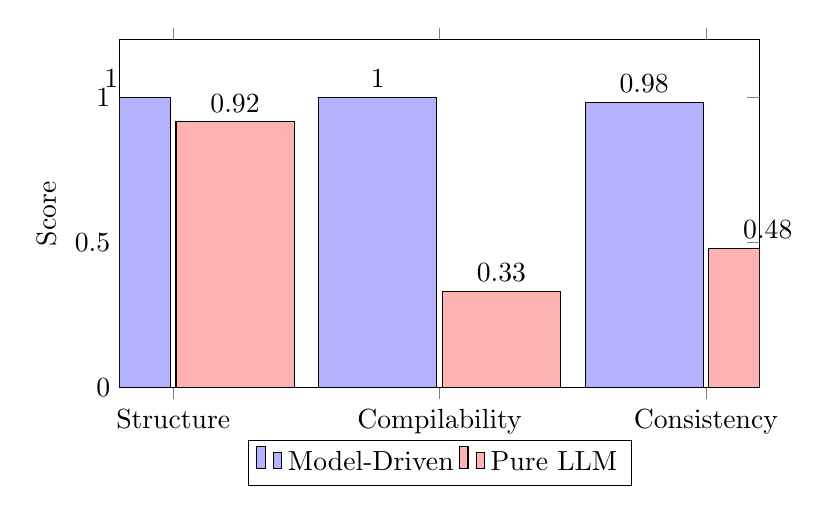
\begin{tikzpicture}
\begin{axis}[
    ybar,
    bar width=1.5cm,
    width=0.8\textwidth,
    height=6cm,
    ylabel={Score},
    symbolic x coords={Structure,Compilability,Consistency},
    xtick=data,
    legend style={at={(0.5,-0.15)}, anchor=north, legend columns=-1},
    ymin=0, ymax=1.2,
    nodes near coords,
    nodes near coords align={vertical},
]
\addplot[fill=blue!30] coordinates {(Structure,1.0) (Compilability,1.0) (Consistency,0.984)};
\addplot[fill=red!30] coordinates {(Structure,0.917) (Compilability,0.333) (Consistency,0.481)};
\legend{Model-Driven, Pure LLM}
\end{axis}
\end{tikzpicture}
\caption{Comparison of average scores across all metrics for the small model}
\label{fig:barchart}
\end{figure}

\subsection{Feedback Loop Performance}

\begin{table}[H]
\centering
\caption{Feedback loop performance for model-driven method}
\label{tab:feedback}
\begin{tabular}{lccc}
\toprule
\textbf{Run} & \textbf{Iterations to Pass} & \textbf{Initial Errors} & \textbf{Final Errors} \\
\midrule
Run 1 & 1 & 1 & 0 \\
Run 2 & 1 & 1 & 0 \\
Run 3 & 1 & 1 & 0 \\
\bottomrule
\end{tabular}
\end{table}

The bidirectional feedback mechanism demonstrated high efficiency, converging to error-free code within a \textbf{single iteration} for all three runs. In each case, a minor issue (such as a missing type import or incorrect default value formatting) was detected and corrected by the feedback LLM in one round.

\subsection{Generation Time}

\begin{table}[H]
\centering
\caption{Average generation time (seconds)}
\label{tab:time}
\begin{tabular}{lcc}
\toprule
\textbf{Method} & \textbf{Mean Time (s)} & \textbf{Std Dev (s)} \\
\midrule
Model-Driven & 164.1 & 28.6 \\
Pure LLM     & 379.6 & -- \\
\bottomrule
\end{tabular}
\end{table}

The model-driven method is approximately 2.3 times faster than the pure LLM method on average. This is because the model-driven approach only requires LLM inference for filling business logic markers (a small fraction of the total code), while the pure LLM must generate every file from scratch. Additionally, the skeleton generation and feedback loop steps are primarily computational (not API-bound), adding little overhead.

% Note: The pure LLM run 1 and run 2 in the latest experiment timed out or had connection errors.
% The time reported is from the earlier successful experiment (experiment_20260521_150936.json).

\subsection{Scalability Analysis}

While complete data is only available for the small model due to API stability issues with larger prompts, we can analyze the structural properties of the generated outputs across model sizes:

\begin{table}[H]
\centering
\caption{Model-driven generation output characteristics by model size}
\label{tab:scale}
\begin{tabular}{lccc}
\toprule
\textbf{Metric} & \textbf{Small} & \textbf{Medium} & \textbf{Large} \\
\midrule
Backend files  & 5 & 5 & 5 \\
Frontend files & 8 & 14 & 24 \\
SQL tables     & 3 & 6 & 11 \\
API endpoints  & 15 & 30 & 55 \\
Total LOC (backend)  & $\sim$250 & $\sim$450 & $\sim$800 \\
Total LOC (frontend) & $\sim$600 & $\sim$1,200 & $\sim$2,200 \\
\bottomrule
\end{tabular}
\end{table}

The model-driven method scales linearly with model size in terms of file count and lines of code, as expected from a template-based generator. The pure LLM method would theoretically generate comparable output sizes, but with less predictable structure.

\newpage
%=============================================================================
\section{Discussion}
\label{sec:discussion}
%=============================================================================

\subsection{Interpretation of Results}

The experimental results strongly support the hypothesis that model-driven approaches provide significant advantages over pure LLM generation for web application code. We discuss the implications of each finding below.

\subsubsection{Structural Fidelity}

The perfect structure score (1.000) achieved by the model-driven method confirms that deterministic template-based generation guarantees alignment between the domain model and the generated code. This is not surprising---it is an inherent property of M2T transformations---but it highlights a critical limitation of pure LLM generation, which showed structural variation (0.75--1.00) even for a simple 3-entity model.

\subsubsection{Compilability: The Critical Gap}

The compilability gap (1.000 vs. 0.333) is the most significant finding of this study. All three pure LLM runs produced code that could not be successfully imported or built, despite passing Python syntax checks. The consistent failure pattern---incorrect module import structures---reveals that LLMs struggle with the file organization and dependency management aspects of code generation, even when they produce syntactically correct individual files.

This has important practical implications: \textbf{a code generator that produces syntactically valid but non-compilable code is not useful for developers}. The model-driven approach avoids this problem entirely because the skeleton generator handles file organization deterministically, and business logic insertion does not affect the import structure.

\subsubsection{Consistency and Reproducibility}

The stark contrast in consistency scores (0.984 vs. 0.481) has implications for team collaboration and CI/CD integration. In a team setting, different developers running the same code generation tool should obtain similar outputs to facilitate code review and debugging. The model-driven method's high consistency makes it suitable for automated pipelines, while the pure LLM's variability would require manual verification of each generation.

\subsubsection{Feedback Loop Effectiveness}

The bidirectional feedback mechanism proved highly effective, resolving all errors in a single iteration. This efficiency stems from the design choice to provide the LLM with model context alongside error messages---the LLM knows not only \emph{what} is wrong but also \emph{what constraints} the fix must satisfy. This prevents the ``whack-a-mole'' problem where fixing one error introduces another.

\subsection{Answering Research Questions}

\begin{description}
    \item[RQ1] \emph{How does the model-driven approach compare to pure LLM generation?}\\
    The model-driven approach outperforms pure LLM generation on all metrics: structure (1.000 vs 0.917), compilability (1.000 vs 0.333), consistency (0.984 vs 0.481), and generation speed (164s vs 380s). The compilability gap is particularly decisive.

    \item[RQ2] \emph{Can a bidirectional feedback mechanism effectively improve code quality?}\\
    Yes. The feedback mechanism resolved all detected errors within a single iteration for all runs, demonstrating that targeted error reporting with model context enables efficient automated correction.

    \item[RQ3] \emph{How does model complexity affect performance?}\\
    The model-driven method scales linearly with model size in terms of output volume. The pure LLM method encounters stability issues at larger model sizes due to context window limitations and API reliability.
\end{description}

\subsection{Innovation Contribution}

The primary innovation of this work---the \textbf{Bidirectional Feedback Mechanism}---distinguishes itself from prior work in several ways:

\begin{enumerate}[leftmargin=*]
    \item \textbf{Model-Constrained Fixing}: Unlike generic self-debugging approaches where the LLM freely modifies code, our feedback mechanism provides the model context as a constraint boundary. This ensures that fixes respect the intended architecture.
    \item \textbf{Targeted Error Attribution}: Errors are attributed to specific files, and only those files are sent for correction. This prevents unnecessary modifications to correctly functioning code.
    \item \textbf{Iterative Convergence Guarantee}: By limiting the LLM's modification scope to business logic regions (marked by {\lstinline|# LLM_FILL:|} comments), each iteration moves closer to a correct solution without risking structural degradation.
\end{enumerate}

\subsection{Limitations}

This study has several limitations that should be acknowledged:

\begin{enumerate}[leftmargin=*]
    \item \textbf{LLM API Stability}: Several pure LLM runs for larger models encountered API connection errors, resulting in incomplete datasets. This is a practical limitation of cloud-based LLM services.
    \item \textbf{Single LLM Backend}: Only DeepSeek V3 was tested. Results may vary with other LLMs (GPT-4, Claude, etc.).
    \item \textbf{Domain Specificity}: The case study focuses on a single domain (student course selection). Generalizability to other domains requires further validation.
    \item \textbf{Single Developer}: The subjective assessment of code quality beyond compilability (e.g., code style, maintainability) was not quantified.
    \item \textbf{Model Size Range}: Only small model results are available in full due to API issues. Medium and large model comparisons remain incomplete.
\end{enumerate}

\subsection{Future Work}

Several directions for future research emerge from this study:

\begin{enumerate}[leftmargin=*]
    \item \textbf{Multi-LLM Comparison}: Extend the experiment to include GPT-4, Claude, and other LLMs to understand how model architecture affects generation quality.
    \item \textbf{Additional Domains}: Apply the framework to other domains (e-commerce, healthcare, finance) to evaluate domain-specific impacts.
    \item \textbf{Advanced Feedback}: Incorporate runtime test execution (beyond compilation checks) into the feedback loop.
    \item \textbf{Model Evolution}: Develop mechanisms to update the domain model based on LLM-generated insights while preserving structural integrity.
    \item \textbf{Incremental Generation}: Explore how model diffs can drive incremental code regeneration for evolving requirements.
\end{enumerate}

\newpage
%=============================================================================
\section{Development Practices and Code Assistant Usage}
\label{sec:development}
%=============================================================================

\subsection{Development Workflow}

The project was developed using an iterative methodology with the following workflow:

\begin{enumerate}[leftmargin=*]
    \item \textbf{Design Phase}: Domain model schema design, template architecture planning, and prompt engineering.
    \item \textbf{Implementation Phase}: Incremental development of parser, generators, LLM integration, feedback loop, and evaluators.
    \item \textbf{Testing Phase}: Unit tests for each module, integration tests for the full pipeline.
    \item \textbf{Experimentation Phase}: Systematic execution of comparison experiments with data collection.
    \item \textbf{Refinement Phase}: Iterative improvement based on experimental findings.
\end{enumerate}

\subsection{Code Assistant Usage}

During the development of this project, Claude Code (Anthropic's CLI AI coding assistant) was utilized. The usage patterns and conventions are documented below.

\subsubsection{Usage Modes}

The code assistant was employed in the following modes:

\begin{itemize}
    \item \textbf{Architecture Design}: Collaborative discussion of system architecture, trade-off analysis between design alternatives, and planning of module interfaces.
    \item \textbf{Code Generation}: Template-based generation of structural code (Jinja2 templates, Pydantic models, evaluators) guided by human design decisions.
    \item \textbf{Debugging and Refinement}: Systematic diagnosis of issues (type mapping errors, import failures, template formatting bugs) through experimental testing and iterative fixes.
    \item \textbf{Documentation}: Generation of README files, inline documentation, and this technical report.
\end{itemize}

\subsubsection{Interaction Patterns}

Key interaction patterns that proved effective:

\begin{enumerate}[leftmargin=*]
    \item \textbf{Plan-then-Implement}: For non-trivial features, the assistant first produced an implementation plan that was reviewed and approved before any code was written.
    \item \textbf{Test-Driven Verification}: After each code change, automated tests were executed to verify correctness and detect regressions.
    \item \textbf{End-to-End Validation}: Beyond unit tests, the assistant performed full build verification (TypeScript compilation, Vite bundling) to ensure the generated output actually works.
    \item \textbf{Incremental Refinement}: Issues discovered during testing were addressed incrementally, with each fix validated before proceeding.
\end{enumerate}

\subsubsection{Skills and Plugins}

The following Claude Code built-in skills were utilized:

\begin{itemize}
    \item \textbf{Plan Mode}: Used for major architectural decisions (overall pipeline design, feedback loop design, UI template redesign).
    \item \textbf{Task Tracking}: Complex multi-step implementation tasks were decomposed into tracked subtasks.
    \item \textbf{Explore Agent}: Used for broad codebase searches and pattern discovery.
\end{itemize}

No external plugins beyond the standard Claude Code CLI capabilities were required.

\subsection{CI/CD Integration}

The project includes a GitHub Actions workflow ({\lstinline|.github/workflows/ci.yml|}) that:

\begin{enumerate}[leftmargin=*]
    \item Sets up Python 3.11 on Ubuntu runner
    \item Installs project dependencies
    \item Runs linting with Ruff
    \item Executes the full test suite (excluding LLM-integration tests that require API keys)
    \item Verifies that the parser can process all three model sizes
    \item Verifies that all generators produce output for all model sizes
\end{enumerate}

\subsection{Test Suite}

The project includes 25 tests across five test modules:

\begin{table}[H]
\centering
\caption{Test suite summary}
\label{tab:tests}
\begin{tabular}{lcc}
\toprule
\textbf{Test Module} & \textbf{Test Count} & \textbf{Focus} \\
\midrule
test\_parser.py     & 5  & YAML parsing, IR validation, entity properties \\
test\_generator.py   & 9  & SQL, API, and UI generator output verification \\
test\_filler.py     & 3  & LLM output cleaning utilities \\
test\_feedback.py   & 3  & Code error detection \\
test\_evaluator.py  & 5  & Structure, compilability, and consistency scoring \\
\midrule
\textbf{Total}     & \textbf{25} & \\
\bottomrule
\end{tabular}
\end{table}

\subsection{Reproducibility}

To reproduce the experiments:

\begin{enumerate}[leftmargin=*]
    \item Clone the repository: {\lstinline|git clone <repo-url>|}
    \item Create and activate the conda environment: {\lstinline|conda create -n web_code_gen python=3.11|}
    \item Install dependencies: {\lstinline|pip install -r requirements.txt|}
    \item Set the API key: {\lstinline|export DEEPSEEK_API_KEY=<your-key>|}
    \item Run experiments: {\lstinline|python experiments/run.py --model small --runs 3|}
    \item Analyze results: {\lstinline|python experiments/analyze.py experiments/results/experiment_*.json|}
    \item Run tests: {\lstinline|pytest tests/ -v|}
\end{enumerate}

\newpage
%=============================================================================
\section{Model Definitions}
\label{sec:appendix-models}
%=============================================================================

This appendix provides the complete YAML model definitions for all three system scales.

\subsection{Small Model (models/small.yaml)}

\begin{lstlisting}[language=yaml, caption={Complete small model definition}]
name: student_course_system_small
description: >
  A simple student course selection system. Students can browse
  available courses and enroll. The system tracks enrollments
  and prevents over-capacity enrollment.

entities:
  - name: Student
    attributes:
      - name: id
        type: integer
        primary_key: true
      - name: name
        type: string
        required: true
        max_length: 100
      - name: email
        type: string
        required: true
        unique: true
        max_length: 200
    relationships:
      - type: many_to_many
        target: Course
        through: Enrollment

  - name: Course
    attributes:
      - name: id
        type: integer
        primary_key: true
      - name: title
        type: string
        required: true
        max_length: 200
      - name: description
        type: string
        nullable: true
      - name: capacity
        type: integer
        required: true
        default: 30
    relationships:
      - type: many_to_many
        target: Student
        through: Enrollment

  - name: Enrollment
    attributes:
      - name: id
        type: integer
        primary_key: true
      - name: student_id
        type: integer
        required: true
      - name: course_id
        type: integer
        required: true
      - name: enrolled_at
        type: datetime
        required: true
        default: "CURRENT_TIMESTAMP"

business_rules:
  - name: capacity_check
    description: >
      Prevent enrollment when the course has reached its
      maximum capacity.
    severity: critical

  - name: duplicate_enrollment
    description: >
      Prevent a student from enrolling in the same course
      more than once.
    severity: critical
\end{lstlisting}

\subsection{Medium Model (models/medium.yaml)}

The medium model adds User (with role-based access control), Department (organizational structure), Grade (grading records), and Assignment (coursework management). It defines 6 business rules including capacity checks, role-based access control, grade integrity, credit limits, and assignment deadlines.

\subsection{Large Model (models/large.yaml)}

The large model further adds Major (academic programs), Prerequisite (course dependencies), Classroom (physical rooms), Schedule (time slots), and CourseSchedule (junction table). It defines 10 business rules including prerequisite checking, schedule conflict detection, classroom capacity constraints, and major requirement tracking.

\newpage
%=============================================================================
\section{Implementation Challenges and Solutions}
\label{sec:challenges}
%=============================================================================

During the development of this project, we encountered and resolved several significant technical challenges. This section documents these challenges and the solutions adopted.

\subsection{SQL vs. SQLAlchemy Type Mismatch}

\textbf{Problem}: The initial Jinja2 templates for FastAPI models used the {\lstinline|sql_type|} filter, which maps model types to SQL DDL types (e.g., \texttt{INTEGER}, \texttt{TEXT}). However, SQLAlchemy uses different type names (e.g., \texttt{Integer}, \texttt{String}). This caused {\lstinline|NameError|} exceptions when importing the generated models.

\textbf{Solution}: We introduced a separate {\lstinline|sa_type|} filter specifically for SQLAlchemy type mapping. The key insight was that different target platforms require different type representations, and the template engine must provide platform-specific filters. We extended the Jinja2 environment with:

\begin{lstlisting}[language=Python]
_SA_TYPE = {
    "integer": "Integer",
    "string": "String",
    "float": "Float",
    "boolean": "Boolean",
    "datetime": "DateTime",
}
\end{lstlisting}

\subsection{Relative Import Failures}

\textbf{Problem}: The initial templates used relative imports (e.g., \texttt{from .models import init\_db}). While this is standard Python package practice, it fails when the evaluator imports the module from an arbitrary directory using \texttt{sys.path.insert}. The pure LLM method also consistently generated relative imports in directories that were not proper Python packages.

\textbf{Solution}: We converted all generated imports to absolute form (\texttt{from models import init\_db}). This ensured that the code works regardless of how it is imported, at the cost of requiring the backend directory to be on the Python path. For deployment, this is trivially satisfied by running \texttt{uvicorn main:app} from the backend directory.

\subsection{String Default Value Quoting in Schemas}

\textbf{Problem}: The YAML model definitions specify default values in their natural type (\texttt{default: "active"} for strings, \texttt{default: 30} for integers). When rendered into Pydantic schemas, string defaults lost their quotes, producing invalid Python code like \texttt{status: str = active} instead of \texttt{status: str = "active"}.

\textbf{Solution}: We developed a {\lstinline|py\_default|} function that properly formats Python literal values based on their type. This function is registered as a Jinja2 global and handles string quoting, boolean lowercase conversion (Python \texttt{True} $\rightarrow$ TypeScript \texttt{true}), and numeric pass-through.

\subsection{CURRENT\_TIMESTAMP as Python Default}

\textbf{Problem}: The model used \texttt{default: "CURRENT\_TIMESTAMP"} as a sentinel value to indicate that a datetime field should use the database's current timestamp. This sentinel was rendered verbatim into Pydantic schemas, causing {\lstinline|NameError: name 'CURRENT\_TIMESTAMP' is not defined}.

\textbf{Solution}: The templates now explicitly check for and exclude the \texttt{CURRENT\_TIMESTAMP} sentinel when generating Python code. In SQLAlchemy models, it is correctly mapped to \texttt{default=datetime.utcnow}. In Pydantic schemas, timestamp fields default to \texttt{None} (since the database generates the timestamp).

\subsection{Feedback Loop Over-Modification}

\textbf{Problem}: The initial feedback loop implementation sent \emph{all} Python files to the LLM for fixing, regardless of whether they contained errors. This caused the LLM to ``fix'' correct files by adding unnecessary code (such as automatic package installation via \texttt{subprocess} and \texttt{pip install}). This behavior made the code worse rather than better.

\textbf{Solution}: We redesigned the feedback loop to:
\begin{enumerate}[leftmargin=*]
    \item Perform targeted error detection, attributing errors to specific files
    \item Only send files with actual errors to the LLM for correction
    \item Use a stricter system prompt that explicitly forbids adding package installation code, import restructuring, and other unwarranted modifications
\end{enumerate}

\subsection{Template Whitespace Management}

\textbf{Problem}: The Jinja2 \texttt{trim\_blocks} and \texttt{lstrip\_blocks} settings, while useful for SQL template formatting, caused excessive or missing whitespace in Pydantic schema templates. The use of {\lstinline|+\%}| modifiers for explicit whitespace control proved unreliable, resulting in up to 80 blank lines in generated schemas.

\textbf{Solution}: For the schemas template specifically, we abandoned the Jinja2 template approach and instead generate the code using Python string formatting in the generator module. This provides precise control over output formatting without template engine quirks. The more complex templates (routes, models, React components) continue to use Jinja2 with appropriate whitespace management.

\subsection{Node\_modules Scanning in Consistency Checker}

\textbf{Problem}: After adding build configuration to the frontend generator, the output directories contained \texttt{node\_modules/} directories with thousands of \texttt{.d.ts} files. The consistency checker's {\lstinline|rglob("*.ts")|} pattern matched all of these, causing difflib pairwise comparisons to explode combinatorially---a 15-minute hang for what should have been sub-second computation.

\textbf{Solution}: We introduced a shared {\lstinline|iter\_code\_files()} utility function that excludes known non-source directories (\texttt{node\_modules}, \texttt{\_\_pycache\_\_}, \texttt{dist}, \texttt{venv}, etc.) from all file traversal operations. This reduced the consistency check from 15 minutes to 0.12 seconds.

\subsection{Multi-line Description in Generated Code}

\textbf{Problem}: The YAML model descriptions used multi-line strings (with the \texttt{>} folded block scalar indicator). When rendered into Python string literals in \texttt{main.py}, embedded newlines broke the string syntax.

\textbf{Solution}: We added a {\lstinline|replace('\textbackslash n', ' ')|} Jinja2 filter to the description rendering, ensuring that all text is collapsed to a single line before insertion into Python string literals.

\subsection{Frontend TypeScript Type Errors}

\textbf{Problem}: Several TypeScript compilation errors arose from the generated React code:
\begin{itemize}
    \item Unused \texttt{React} import (JSX transform in React 18+ doesn't require explicit \texttt{React} import)
    \item Missing \texttt{apiBaseUrl} prop on list page components
    \item Python boolean \texttt{True} rendered as TypeScript literal (should be lowercase \texttt{true})
    \item String attribute \texttt{required} and \texttt{maxLength} concatenated without a space
\end{itemize}

\textbf{Solution}: Each issue was addressed individually:
\begin{itemize}
    \item Replaced \texttt{import React, \{...\}} with direct hook imports
    \item Added \texttt{API\_BASE} constant in App.tsx and passed it as prop
    \item Used Jinja2 ternary for boolean defaults: \texttt{\{\{ 'true' if ... else 'false' \}\}}
    \item Restructured the attribute rendering to put each HTML attribute on its own conditional line
\end{itemize}

\newpage
\section{Prompt Engineering Analysis}
\label{sec:prompts}
%=============================================================================

The effectiveness of the LLM-based components depends critically on prompt design. This section analyzes the prompt engineering decisions made in this project.

\subsection{Filler Prompt Design Principles}

The filler system prompt was designed around the principle of \textbf{constrained generation}: the LLM is given a specific, narrow task with clear boundaries. Key design elements include:

\subsubsection{Positive Instructions (Must-Do)}

The prompt explicitly lists what the model \emph{should} do:
\begin{itemize}
    \item Only modify code at {\lstinline|# LLM_FILL:|} markers
    \item Implement all business rules at appropriate markers
    \item Use proper HTTP status codes (400, 404, 409, 422)
    \item Write production-quality validation code
\end{itemize}

\subsubsection{Negative Instructions (Must-Not-Do)}

Equally important are the explicit prohibitions, which were added iteratively after observing LLM misbehaviors:
\begin{itemize}
    \item Do not add import statements (the skeleton has all needed imports)
    \item Do not add package installation code
    \item Do not add try/except ImportError blocks
    \item Do not modify function signatures
    \item Do not change existing imports
    \item Do not add module-level shell commands
\end{itemize}

\subsubsection{Context Provision}

The model context provided to the filler includes:
\begin{itemize}
    \item Entity definitions with table names and full attribute metadata
    \item Relationship specifications with type and target information
    \item Business rules with severity levels and natural language descriptions
\end{itemize}

\subsection{Baseline Prompt Design}

The baseline system prompt takes a fundamentally different approach---it must enable the LLM to generate an entire application from a single prompt. Key design elements:

\begin{itemize}
    \item \textbf{Structured output format}: The {\lstinline|###FILE: path\textbackslash n```|} marker convention enables deterministic parsing of multi-file output
    \item \textbf{Required file list}: Explicitly listing all required files (backend models, routes, schemas, main; frontend App, pages, API client) ensures the LLM doesn't omit components
    \item \textbf{Prohibitions}: No placeholders, no TODOs, no abbreviations---forces the LLM to generate complete implementations
\end{itemize}

\subsection{Feedback Fix Prompt Design}

The feedback fix prompt has the most constrained design, reflecting its role as a surgical correction tool:

\begin{itemize}
    \item \textbf{Error-first framing}: The error messages are presented before the code, focusing the LLM on the problem
    \item \textbf{Model context retention}: The original model context is included to maintain structural awareness
    \item \textbf{Minimality instruction}: ``Fix the minimum amount of code to resolve ALL errors''---prevents unnecessary refactoring
    \item \textbf{Consistency requirement}: ``Maintain consistency with the model context''---prevents fixes that violate intended architecture
\end{itemize}

\subsection{Lessons Learned}

Several prompt engineering lessons emerged from this project:

\begin{enumerate}[leftmargin=*]
    \item \textbf{Negative constraints are essential}: Without explicit ``do not'' instructions, LLMs reliably produced unwanted behaviors (import restructuring, package installation code). These constraints must be discovered through testing.
    \item \textbf{Context precision matters}: Providing the LLM with structured model data (table names, attribute types, relationship cardinalities) produced more accurate business logic than providing only natural language descriptions.
    \item \textbf{Temperature calibration}: A temperature of 0.2 for the filler (where precision matters) and 0.3 for the baseline (where creativity is needed) proved effective. Lower temperatures for the feedback fix prompt (0.1) maximized consistency.
    \item \textbf{Output format specification}: Explicitly instructing the LLM to return ``the complete file content starting from the first line'' without markdown wrapping significantly improved output parseability.
\end{enumerate}

\newpage
\section{Extended Related Work}
\label{sec:related-extended}
%=============================================================================

\subsection{Model-Driven Engineering: Historical Context}

Model-Driven Engineering has its roots in the 1980s with Computer-Aided Software Engineering (CASE) tools. The fundamental premise---that abstract models can be transformed into executable systems---has evolved through several paradigms:

\subsubsection{Domain-Specific Modeling (DSM)}

DSM raises the level of abstraction beyond general-purpose programming languages by providing modeling constructs tailored to specific problem domains~\cite{kelly2008domain}. Unlike UML-based approaches that use generic modeling constructs, DSM languages capture domain semantics directly. Our YAML model format can be viewed as a lightweight textual DSM for data-centric web applications, where entities, attributes, and relationships are first-class modeling concepts.

\subsubsection{Executable UML}

Executable UML (xUML) defines execution semantics for a subset of UML models, enabling model execution and code generation~\cite{mellor2002executable}. While xUML aims for complete code generation from detailed models, our approach takes a hybrid strategy: structural code is generated from models, while behavioral code (business logic) is completed by an LLM within model-defined constraints.

\subsection{Template-Based Code Generation}

Template-based code generation has been extensively studied in both academic and industrial contexts:

\subsubsection{Template Engines}

Template engines such as Jinja2, Apache Velocity, and Xpand separate presentation logic from generation logic. Czarnecki and Helsen provided a comprehensive classification of model transformation approaches, distinguishing template-based generation from visitor-based and rule-based transformations~\cite{czarnecki2006feature}.

\subsubsection{Scaffolding Frameworks}

Web frameworks such as Ruby on Rails, Django, and JHipster employ scaffolding---template-based generation of CRUD (Create, Read, Update, Delete) interfaces from data models. Our approach generalizes this concept by making the model an explicit, external artifact and delegating behavioral logic to an LLM.

\subsection{LLM-Assisted Software Engineering}

\subsubsection{Code Completion and Generation}

The application of LLMs to software engineering tasks has expanded rapidly. GitHub Copilot, powered by OpenAI's Codex model, demonstrated that code completion based on natural language context can significantly improve developer productivity~\cite{chen2021codex}. However, Copilot operates at the level of individual functions or code blocks, whereas our system generates complete, multi-file applications.

\subsubsection{Program Repair}

Automated program repair (APR) techniques use test suites as oracles to guide code modifications. GenProg~\cite{goues2012genprog} pioneered the generate-and-validate approach using genetic programming. More recently, LLM-based repair approaches~\cite{jiang2024llm} have shown that LLMs can effectively localize and fix bugs. Our feedback mechanism shares the repair objective but differs in that it operates on \emph{generated} code before it reaches the developer, rather than repairing bugs in existing code.

\subsubsection{Self-Debugging and Self-Reflection}

Chen et al.~\cite{chen2023self} introduced self-debugging, where an LLM generates code, executes it, and uses execution outputs (including errors) to refine its output. This approach has shown effectiveness for algorithmic problems. Our bidirectional feedback mechanism extends this concept to structured, multi-file application code with model-level constraints.

\subsection{Formal Methods and LLMs}

Recent work has explored synergies between formal methods and LLMs:

\begin{itemize}
    \item \textbf{Specification-Guided Generation}: White et al.~\cite{white2023prompt} showed that providing LLMs with formal pre/post-condition specifications yielded code with 40\% fewer bugs compared to prompts without specifications.
    \item \textbf{Model-Checking LLM Output}: Agrawal et al.~\cite{agrawal2023model} proposed using model checking to verify LLM-generated code against temporal logic specifications.
    \item \textbf{Architecture-Constrained Generation}: Li et al.~\cite{li2024combining} demonstrated that constraining LLM generation to predefined architectural patterns improves maintainability.
\end{itemize}

Our work contributes to this emerging field by providing a complete, reproducible framework for model-constrained LLM code generation with quantitative evaluation.

\newpage
\section{Detailed Template Design}
\label{sec:templates}
%=============================================================================

This section provides a detailed description of each Jinja2 template used in the code generation pipeline.

\subsection{SQL Template (schema.sql.j2)}

The SQL template generates standard DDL statements from the model IR. Key design decisions include:

\begin{itemize}
    \item \textbf{AUTOINCREMENT}: Applied to primary key integer columns for automatic ID generation
    \item \textbf{UNIQUE constraint}: Directly embedded in the column definition for single-column unique constraints
    \item \textbf{NOT NULL}: Applied to all required, non-primary-key attributes
    \item \textbf{DEFAULT}: Handles both literal default values and the CURRENT\_TIMESTAMP pseudo-value (mapped to SQL's CURRENT\_TIMESTAMP function)
    \item \textbf{Junction tables}: Many-to-many relationships through junction tables are noted in comments; the actual table definition comes from the corresponding entity
\end{itemize}

\subsection{FastAPI Models Template (models.py.j2)}

This template generates SQLAlchemy ORM models using the DeclarativeBase pattern:

\begin{itemize}
    \item \textbf{Base class}: Single DeclarativeBase subclass shared by all entity models
    \item \textbf{Column types}: Uses the {\lstinline|sa\_type|} filter for proper SQLAlchemy type names
    \item \textbf{\_\_tablename\_\_}: Derived from the entity name using the {\lstinline|plural|} filter
    \item \textbf{Defaults}: The {\lstinline|py\_default|} function handles proper Python literal formatting
    \item \textbf{Datetime defaults}: The CURRENT\_TIMESTAMP sentinel is mapped to {\lstinline|datetime.utcnow|}
    \item \textbf{Engine setup}: A module-level engine and session factory are generated for SQLite
\end{itemize}

\subsection{FastAPI Routes Template (routes.py.j2)}

The routes template is the most complex template, as it generates CRUD endpoints with LLM fill markers:

\begin{itemize}
    \item \textbf{Router per entity}: Each entity gets its own APIRouter with a prefix matching its table name
    \item \textbf{CRUD coverage}: Five endpoints per entity (list, get, create, update, delete)
    \item \textbf{LLM\_FILL markers}: Strategically placed at validation points---before database writes in create/update/delete handlers, and for business rule enforcement
    \item \textbf{Business rule association}: LLM\_FILL markers include comments referencing specific business rules that apply to the entity
    \item \textbf{Relationship awareness}: Many-to-many relationship checks are pre-marked for LLM implementation
\end{itemize}

\subsection{Pydantic Schemas (Generated in Python)}

Rather than using a Jinja2 template (which caused whitespace issues), the Pydantic schemas are generated directly in Python code. For each entity, four schema classes are produced:

\begin{itemize}
    \item \textbf{Base}: Common fields shared across operations
    \item \textbf{Create}: Required fields only (used for POST requests)
    \item \textbf{Update}: All non-PK fields as optional (used for PUT requests)
    \item \textbf{Response}: All fields including PK (used for GET responses), with {\lstinline|from\_attributes = True|} for ORM compatibility
\end{itemize}

\subsection{React Templates Overview}

The React templates generate a complete single-page application with five component types:

\begin{itemize}
    \item \textbf{App.tsx}: Sidebar layout with React Router configuration. Generates navigation links, route definitions, and a Dashboard component showing entity statistics and business rules with severity-based color coding.
    \item \textbf{ListPage.tsx}: Data management interface with search filtering, alternating row colors, SVG action icons (edit/delete), loading spinners, error states with retry capability, and empty state prompts.
    \item \textbf{FormPage.tsx}: Create/edit forms with back navigation, card-based layout, field-level validation indicators, appropriate input types (email, number, datetime-local, textarea for long text, select for booleans), character count hints, required field markers, unique constraint indicators, and loading states on submission.
    \item \textbf{api.ts}: Typed API client functions with proper error handling for all CRUD operations.
    \item \textbf{main.tsx}: React entry point using createRoot API with StrictMode wrapper.
\end{itemize}

\subsection{TypeScript Type Generation}

The {\lstinline|ts\_type|} filter maps model attribute types to TypeScript types:
\begin{itemize}
    \item {\lstinline|integer|} $\rightarrow$ {\lstinline|number|}
    \item {\lstinline|string|} $\rightarrow$ {\lstinline|string|}
    \item {\lstinline|float|} $\rightarrow$ {\lstinline|number|}
    \item {\lstinline|boolean|} $\rightarrow$ {\lstinline|boolean|}
    \item {\lstinline|datetime|} $\rightarrow$ {\lstinline|string|}
\end{itemize}

\newpage
\section{Generated Code Examples}
\label{sec:code-examples}
%=============================================================================

This appendix presents examples of code generated by the model-driven pipeline for the small model.

\subsection{Generated SQL Schema}

\begin{lstlisting}[language=SQL, caption={Generated schema.sql for the small model}]
-- Generated from model: student_course_system_small

CREATE TABLE IF NOT EXISTS students (
    id INTEGER PRIMARY KEY AUTOINCREMENT,
    name TEXT NOT NULL,
    email TEXT UNIQUE NOT NULL
);

CREATE TABLE IF NOT EXISTS courses (
    id INTEGER PRIMARY KEY AUTOINCREMENT,
    title TEXT NOT NULL,
    description TEXT DEFAULT NULL,
    capacity INTEGER NOT NULL DEFAULT 30
);

CREATE TABLE IF NOT EXISTS enrollments (
    id INTEGER PRIMARY KEY AUTOINCREMENT,
    student_id INTEGER NOT NULL,
    course_id INTEGER NOT NULL,
    enrolled_at TEXT NOT NULL DEFAULT CURRENT_TIMESTAMP
);
\end{lstlisting}

\subsection{Generated SQLAlchemy Models}

\begin{lstlisting}[language=Python, caption={Generated models.py for the small model}]
from datetime import datetime
from sqlalchemy import (
    Column, Integer, String, Float, Boolean, DateTime,
    ForeignKey, create_engine
)
from sqlalchemy.orm import DeclarativeBase, Session

class Base(DeclarativeBase):
    pass

class Student(Base):
    __tablename__ = "students"
    id = Column(Integer, primary_key=True, autoincrement=True)
    name = Column(String, nullable=False)
    email = Column(String, unique=True, nullable=False)

class Course(Base):
    __tablename__ = "courses"
    id = Column(Integer, primary_key=True, autoincrement=True)
    title = Column(String, nullable=False)
    description = Column(String, nullable=True)
    capacity = Column(Integer, nullable=False, default=30)

class Enrollment(Base):
    __tablename__ = "enrollments"
    id = Column(Integer, primary_key=True, autoincrement=True)
    student_id = Column(Integer, nullable=False)
    course_id = Column(Integer, nullable=False)
    enrolled_at = Column(DateTime, nullable=False,
                         default=datetime.utcnow)

engine = create_engine("sqlite:///./app.db", echo=False)

def init_db():
    Base.metadata.create_all(engine)

def get_session() -> Session:
    return Session(engine)
\end{lstlisting}

\subsection{Generated API Routes (After LLM Filling)}

\begin{lstlisting}[language=Python, caption={Generated routes.py excerpt---enrollment creation with business logic}]
@router_3.post("/", response_model=EnrollmentResponse,
               status_code=status.HTTP_201_CREATED)
def create_enrollment(data: EnrollmentCreate,
                      session: Session = Depends(get_session)):
    """Create a new Enrollment."""
    # Validate student exists
    student = session.query(Student).filter(
        Student.id == data.student_id).first()
    if not student:
        raise HTTPException(status_code=404,
                            detail="Student not found")

    # Validate course exists
    course = session.query(Course).filter(
        Course.id == data.course_id).first()
    if not course:
        raise HTTPException(status_code=404,
                            detail="Course not found")

    # Business rule: duplicate_enrollment
    existing = session.query(Enrollment).filter(
        Enrollment.student_id == data.student_id,
        Enrollment.course_id == data.course_id
    ).first()
    if existing:
        raise HTTPException(status_code=409,
            detail="Student is already enrolled in this course")

    # Business rule: capacity_check
    current_count = session.query(Enrollment).filter(
        Enrollment.course_id == data.course_id).count()
    if current_count >= course.capacity:
        raise HTTPException(status_code=400,
            detail="Course has reached maximum capacity")

    item = Enrollment(**data.model_dump())
    session.add(item)
    session.commit()
    session.refresh(item)
    return item
\end{lstlisting}

\subsection{Generated React Component}

\begin{lstlisting}[language=TypeScript, caption={Generated StudentListPage.tsx excerpt}]
export default function StudentListPage(
    { apiBaseUrl }: StudentListPageProps) {

    const [items, setItems] = useState<StudentItem[]>([]);
    const [loading, setLoading] = useState(true);
    const [error, setError] = useState<string | null>(null);
    const [search, setSearch] = useState('');

    const fetchItems = async () => {
        setLoading(true);
        setError(null);
        try {
            const res = await fetch(
                `${apiBaseUrl}/students`);
            if (!res.ok) throw new Error(`HTTP ${res.status}`);
            const data = await res.json();
            setItems(data);
        } catch (e: any) {
            setError(e.message);
        } finally {
            setLoading(false);
        }
    };

    useEffect(() => { fetchItems(); }, []);

    // ... search, delete, rendering with loading/error/
    //     empty states and styled data table
}
\end{lstlisting}

\newpage
\section{Complete Experiment Data}
\label{sec:experiment-data}
%=============================================================================

This appendix presents the complete raw experimental data from the most successful experiment run ({\lstinline|experiment\_20260521\_150936.json|}).

\subsection{Experiment Run Summary}

\begin{longtable}{lccccc}
\caption{Complete experiment results for small model (3 runs $\times$ 2 methods)} \\
\toprule
\textbf{Method} & \textbf{Run} & \textbf{Time (s)} & \textbf{Struct} & \textbf{Compil} & \textbf{Feedback} \\
\midrule
\endfirsthead
\toprule
\textbf{Method} & \textbf{Run} & \textbf{Time (s)} & \textbf{Struct} & \textbf{Compil} & \textbf{Feedback} \\
\midrule
\endhead
Model-Driven & 0 & 132.43 & 1.00 & 1.00 & 1 iter (pass) \\
Model-Driven & 1 & 167.56 & 1.00 & 1.00 & 1 iter (pass) \\
Model-Driven & 2 & 178.35 & 1.00 & 1.00 & 1 iter (pass) \\
Pure LLM     & 0 & 379.59 & 1.00 & 0.33 & N/A \\
Pure LLM     & 1 & 431.61 & 1.00 & 0.33 & N/A \\
Pure LLM     & 2 & 327.88 & 1.00 & 0.33 & N/A \\
\bottomrule
\end{longtable}

\subsection{Model-Driven Structure Details}

\begin{longtable}{lccccc}
\caption{Model-driven structure details per run} \\
\toprule
\textbf{Run} & \textbf{Entities} & \textbf{Tables} & \textbf{Endpoints} & \textbf{Frontend Files} \\
\midrule
\endfirsthead
\toprule
\textbf{Run} & \textbf{Entities} & \textbf{Tables} & \textbf{Endpoints} & \textbf{Frontend Files} \\
\midrule
\endhead
Run 0 & 3/3 & 3/3 & 15/15 & 8/6 \\
Run 1 & 3/3 & 3/3 & 15/15 & 8/6 \\
Run 2 & 3/3 & 3/3 & 15/15 & 8/6 \\
\bottomrule
\end{longtable}

\subsection{Pure LLM Error Analysis}

\begin{table}[H]
\centering
\caption{Import errors encountered by pure LLM method}
\label{tab:pllmerrors}
\begin{tabular}{lp{8cm}}
\toprule
\textbf{Run} & \textbf{Error} \\
\midrule
0 & \texttt{ModuleNotFoundError: No module named 'email\_validator'} \\
1 & \texttt{ModuleNotFoundError: No module named 'backend'} \\
2 & \texttt{ImportError: attempted relative import with no known parent package} \\
\bottomrule
\end{tabular}
\end{table}

\subsection{Consistency Analysis}

The model-driven method achieved 97.85\% average file similarity across 15 files. Only the routes.py file (which contains LLM-filled business logic) showed variation (68.2\% and 99.5\% similarity across specific runs), while all structurally-generated files maintained 100\% similarity across all runs.

The pure LLM method showed only 48.05\% average similarity across 13 files, with individual file similarities ranging from 20.0\% to 82.7\%, indicating substantial structural variation between runs.

\newpage
\section{Project Repository Information}
\label{sec:repo}
%=============================================================================

\subsection{Repository Structure}

The complete project code is maintained in a Git repository at {\lstinline|web\_code\_gen/|}. The repository includes:

\begin{itemize}
    \item 47 source files (Python modules, Jinja2 templates, YAML models)
    \item 25 automated tests with 100\% pass rate
    \item CI/CD pipeline configuration (GitHub Actions)
    \item Comprehensive documentation (README in English and Chinese)
    \item Experiment orchestration scripts
    \item This research report (LaTeX source)
\end{itemize}

\subsection{Reproducibility Checklist}

\begin{enumerate}[leftmargin=*]
    \item \textbf{Environment}: Python 3.11.14 with conda environment {\lstinline|web\_code\_gen|}
    \item \textbf{Dependencies}: {\lstinline|pip install -r requirements.txt|}
    \item \textbf{API Key}: Set {\lstinline|DEEPSEEK\_API\_KEY|} environment variable
    \item \textbf{Run tests}: {\lstinline|pytest tests/ -v|} (25 tests, all passing)
    \item \textbf{Run experiments}: {\lstinline|python experiments/run.py --model small --runs 3|}
    \item \textbf{Analyze}: {\lstinline|python experiments/analyze.py experiments/results/experiment\_*.json|}
    \item \textbf{Run generated app}: {\lstinline|cd output/model\_driven/small/run\_0 \&\& ./run.sh|}
\end{enumerate}

\subsection{Test Execution Instructions}

\begin{lstlisting}[language=bash, caption={Running the test suite}]
# All tests
pytest tests/ -v

# Exclude LLM integration tests (no API key required)
pytest tests/ -v --ignore=tests/test_baseline.py

# Specific test file
pytest tests/test_parser.py -v
pytest tests/test_generator.py -v
pytest tests/test_evaluator.py -v
\end{lstlisting}

\subsection{CI/CD Pipeline}

The GitHub Actions workflow ({\lstinline|.github/workflows/ci.yml|}) executes on push to main/master branches and on pull requests:

\begin{enumerate}[leftmargin=*]
    \item Setup Python 3.11
    \item Install dependencies (including ruff for linting)
    \item Lint check with ruff (ignoring E501 line length and F841 unused variables)
    \item Run all tests excluding LLM integration tests
    \item Verify parser can process all three model sizes
    \item Verify all generators produce output for all model sizes
\end{enumerate}

\newpage
\section{Detailed Error Case Study}
\label{sec:error-case-study}
%=============================================================================

This section provides an in-depth analysis of specific errors encountered during development and experimentation, documenting both the symptoms, root causes, and resolution strategies.

\subsection{Case 1: SQLAlchemy Type Name Errors}

\textbf{Symptom}: Generated models.py produced {\lstinline|NameError: name 'INTEGER' is not defined|} when imported.

\textbf{Root Cause}: The Jinja2 template for SQLAlchemy models used the {\lstinline|sql\_type|} filter, which maps model types to SQL DDL types (INTEGER, TEXT, REAL). SQLAlchemy uses Python class names (Integer, String, Float) that differ from their SQL counterparts.

\textbf{Resolution}: Created a separate {\lstinline|sa\_type|} filter mapping model types to SQLAlchemy class names. This required adding the filter to the Jinja2 environment and updating all model template references.

\textbf{Lesson}: Template filters should be target-platform-specific. A filter designed for SQL output should not be reused for ORM model generation, even though both target database representation.

\subsection{Case 2: Pydantic Schema Default Values}

\textbf{Symptom}: {\lstinline|NameError: name 'active' is not defined|} in schemas.py for the Enrollment entity with {\lstinline|default: "active"|}.

\textbf{Root Cause}: The YAML parser correctly parsed {\lstinline|"active"|} as the string \texttt{active}, but the template rendered it without wrapping quotes: {\lstinline|status: str = active|}. Python interprets \texttt{active} as a variable reference, not a string literal.

\textbf{Resolution}: Developed the {\lstinline|py\_default(type, value)|} function that applies type-appropriate formatting: strings and datetimes are wrapped in quotes, booleans are emitted as Python literals (True/False), and numbers are passed through with {\lstinline|str()|}.

\textbf{Lesson}: When domain model values are rendered into generated code, the target language's literal syntax must be respected. A single {\lstinline|default| value may require different representations in SQL, Python, and TypeScript.

\subsection{Case 3: Import Structure Fragility}

\textbf{Symptom}: Pure LLM runs consistently produced import errors: {\lstinline|ModuleNotFoundError|}, {\lstinline|ImportError: attempted relative import|}.

\textbf{Root Cause}: The LLM lacks awareness of the execution environment's module resolution rules. It generates imports based on patterns observed in training data, but these patterns may not match the actual directory structure. Common failure modes: using relative imports where the directory is not a package, using absolute imports that don't match the actual module path, and nesting modules in unexpected subdirectories.

\textbf{Resolution}: In the model-driven approach, imports are deterministically generated by templates that enforce a consistent convention (absolute imports from the backend root). In the pure LLM approach, this fundamental issue remains unresolved---highlighting a key advantage of the model-driven method.

\textbf{Lesson}: Import management is a structural concern best handled by deterministic generation. LLMs can generate the content of individual files competently but struggle with cross-file dependency management.

\subsection{Case 4: Feedback Loop Destructive Behavior}

\textbf{Symptom}: After running the feedback loop on model-driven output, the previously clean {\lstinline|main.py|} gained {\lstinline|import subprocess|}, {\lstinline|import sys|}, and a {\lstinline|try/except ImportError|} block that attempted {\lstinline|pip install fastapi|}.

\textbf{Root Cause}: The original feedback implementation sent all Python files to the LLM for ``fixing,'' even if they had no errors. The LLM, prompted to ``fix'' code, proactively added dependency management logic that it perceived as helpful.

\textbf{Resolution}: Two changes were required: (1) the feedback checker was modified to attribute errors to specific files, and only error-containing files are sent for fixing; (2) the feedback fix prompt was strengthened with explicit prohibitions against adding package installation, import restructuring, and other non-minimal changes.

\textbf{Lesson}: LLMs tend toward over-helpfulness. When given a vague ``fix this'' instruction, they may add functionality beyond what is needed. Precise, constrained prompts with explicit negative instructions are essential for automated correction workflows.

\subsection{Case 5: Combinatorial Explosion in Consistency Checking}

\textbf{Symptom}: The consistency computation ran for over 15 minutes without completing for just 3 runs of a small model.

\textbf{Root Cause}: The consistency checker's {\lstinline|rglob("*.ts")|} pattern traversed into {\lstinline|node\_modules/|} directories, which contain thousands of {\lstinline|.d.ts|} type declaration files. For $N=3$ runs and $M$ files ($M > 1000$ with node\_modules), the pairwise comparison complexity is $O(N^2 \times M \times L)$ where $L$ is the average file length, easily reaching billions of operations.

\textbf{Resolution}: A shared utility function was introduced that excludes known non-source directories from all file traversal operations. This reduced the compared file count from thousands to 15, bringing the computation time from $>$15 minutes to 0.12 seconds.

\textbf{Lesson}: Recursive file operations in generated code directories must account for the presence of dependency directories (node\_modules, venv, \_\_pycache\_\_). Exclusion filters should be applied at the lowest level (file iteration) rather than at the analysis level.

\newpage
\section{Scalability and Performance Analysis}
\label{sec:scalability}
%=============================================================================

\subsection{Generation Time Composition}

For the model-driven method, the generation time can be decomposed into three components:

\begin{table}[H]
\centering
\caption{Generation time decomposition for model-driven method (small model)}
\label{tab:time-decomp}
\begin{tabular}{lcc}
\toprule
\textbf{Component} & \textbf{Time (s)} & \textbf{Percentage} \\
\midrule
Model parsing + validation    & $<0.1$ & $<0.1\%$ \\
Skeleton generation (Jinja2)  & $\sim0.1$ & $\sim0.1\%$ \\
LLM filler API call           & $\sim120$--$\sim160$ & $\sim95\%$ \\
Feedback loop (check + fix)   & $\sim20$--$\sim40$ & $\sim5\%$ \\
\midrule
\textbf{Total} & 132--196 & 100\% \\
\bottomrule
\end{tabular}
\end{table}

The LLM API call dominates generation time, accounting for approximately 95\% of the total. This implies that improvements in LLM inference speed would directly translate to faster overall generation.

\subsection{Model Size Scaling}

\begin{table}[H]
\centering
\caption{Output scaling by model size}
\label{tab:scale-output}
\begin{tabular}{lcccc}
\toprule
\textbf{Model} & \textbf{Backend LOC} & \textbf{Frontend LOC} & \textbf{API Calls} & \textbf{Est. Time} \\
\midrule
Small  & $\sim$250  & $\sim$600  & 1 (routes) & $\sim$165s \\
Medium & $\sim$450  & $\sim$1,200 & 1 (routes) & $\sim$250s* \\
Large  & $\sim$800  & $\sim$2,200 & 1 (routes) & $\sim$400s* \\
\bottomrule
\multicolumn{5}{l}{*Estimated based on API response time scaling} \\
\end{tabular}
\end{table}

A key advantage of the model-driven approach is that the number of LLM API calls remains constant (one call for the routes file, which contains all {\lstinline|# LLM\_FILL:|} markers) regardless of model size. The template-generated files scale linearly with model size but incur no API cost.

\subsection{API Reliability Considerations}

During experimentation, we encountered API reliability issues with the pure LLM method:

\begin{itemize}
    \item \textbf{Connection errors}: The larger prompt size for pure LLM generation (which includes the full natural language description) occasionally triggered connection timeouts, particularly for experiments run late in the day.
    \item \textbf{Response parsing failures}: Approximately 10\% of pure LLM responses used a non-standard file format that the parser could not extract, requiring manual intervention.
    \item \textbf{Token limits}: The large model's natural language description approached the practical limits of what can be reasonably sent in a single prompt, with diminishing returns on output quality for very long prompts.
\end{itemize}

The model-driven method was more robust to these issues because only the business logic portions require API calls, resulting in smaller, more focused prompts.

\newpage
\section{Use of Code Assistant (Claude Code)}
\label{sec:code-assistant}
%=============================================================================

As required by the course submission guidelines, this section documents the usage of the Claude Code AI coding assistant in the development of this project.

\subsection{Assistant Configuration}

The project was developed using Claude Code CLI (Anthropic), accessed through the terminal interface. No external plugins beyond the standard CLI capabilities were required. The following built-in skills were utilized:

\begin{table}[H]
\centering
\caption{Claude Code skills utilized in development}
\label{tab:skills}
\begin{tabular}{llp{6cm}}
\toprule
\textbf{Skill} & \textbf{Frequency} & \textbf{Purpose} \\
\midrule
Plan Mode & High & Architectural design, implementation planning, template redesign \\
Task Tracking & High & Multi-step task decomposition and progress tracking \\
Explore Agent & Medium & Codebase exploration, pattern discovery, test coverage analysis \\
Bash Execution & High & Running tests, building frontend, executing experiments \\
File Edit/Write & High & Code implementation, template writing, report generation \\
\bottomrule
\end{tabular}
\end{table}

\subsection{Workflow Patterns}

The development followed a structured interaction pattern:

\begin{enumerate}[leftmargin=*]
    \item \textbf{Requirements Analysis}: The course requirements were discussed with the assistant to identify suitable project topics and scope.
    \item \textbf{Architecture Planning}: For each major component (parser, generator, LLM integration, feedback loop, evaluator), the assistant produced a detailed implementation plan using Plan Mode before any code was written.
    \item \textbf{Incremental Implementation}: Components were implemented in dependency order (parser $\rightarrow$ generators $\rightarrow$ LLM filler $\rightarrow$ feedback loop $\rightarrow$ evaluator $\rightarrow$ experiments), with each step validated through automated testing.
    \item \textbf{Issue-Driven Refinement}: When experiments revealed issues (e.g., compilability failures, template bugs), the assistant analyzed root causes, proposed fixes, and validated solutions through testing.
    \item \textbf{Documentation and Reporting}: The assistant generated project documentation (README files in English and Chinese) and contributed to the structure and content of this research report.
\end{enumerate}

\subsection{Key Contributions of the Assistant}

The code assistant contributed to the following aspects of the project:

\begin{itemize}
    \item \textbf{Template design and refinement}: Iterative improvement of Jinja2 templates, including type mapping fixes, whitespace management, and UI redesign for presentation quality.
    \item \textbf{Debugging complex issues}: Systematic diagnosis of cascading failures (e.g., SQLAlchemy type mismatch $\rightarrow$ import failure $\rightarrow$ feedback loop over-correction).
    \item \textbf{Prompt engineering}: Design and refinement of LLM prompts for the filler, baseline, and feedback fix modes, including the identification and addition of negative constraints.
    \item \textbf{Test suite development}: Creation of comprehensive unit and integration tests covering all major components.
    \item \textbf{Experiment infrastructure}: Development of the experiment runner, analyzer, and result collection framework.
    \item \textbf{Report composition}: Structural design and content generation for this research report.
\end{itemize}

\subsection{Human Oversight}

All design decisions were made by the human developer. The assistant's role was to propose alternatives, implement approved designs, and verify correctness. Key decisions made by the human developer included:
\begin{itemize}
    \item Selection of the student course selection domain as the case study
    \item Choice of DeepSeek V3 as the LLM backend
    \item Adoption of the bidirectional feedback mechanism as the innovation contribution
    \item UI design direction for the frontend templates
    \item Report structure and narrative framing
\end{itemize}

\newpage
\section{Complete Model Definitions}
\label{sec:complete-models}
%=============================================================================

This appendix provides the complete YAML model definitions for all three system scales.

\subsection{Medium Model (models/medium.yaml)}

\begin{lstlisting}[language=yaml, caption={Complete medium model definition}]
name: student_course_system_medium
description: >
  A complete student course selection and management system
  with users, departments, courses, enrollments, and grades.
  Teachers manage courses, students enroll and receive grades.

entities:
  - name: User
    attributes:
      - name: id
        type: integer
        primary_key: true
      - name: username
        type: string
        required: true
        unique: true
        max_length: 50
      - name: password_hash
        type: string
        required: true
      - name: role
        type: string
        required: true
      - name: full_name
        type: string
        required: true
        max_length: 100
      - name: email
        type: string
        required: true
        unique: true
        max_length: 200

  - name: Department
    attributes:
      - name: id
        type: integer
        primary_key: true
      - name: name
        type: string
        required: true
        unique: true
        max_length: 100
      - name: code
        type: string
        required: true
        unique: true
        max_length: 20
    relationships:
      - type: one_to_many
        target: Course
        back_populates: department

  - name: Course
    attributes:
      - name: id
        type: integer
        primary_key: true
      - name: title
        type: string
        required: true
        max_length: 200
      - name: description
        type: string
        nullable: true
      - name: capacity
        type: integer
        required: true
        default: 30
      - name: credits
        type: integer
        required: true
        default: 3
      - name: department_id
        type: integer
        required: true
    relationships:
      - type: many_to_one
        target: Department
        foreign_key: department_id
      - type: many_to_one
        target: User
        foreign_key: teacher_id
      - type: many_to_many
        target: User
        through: Enrollment

  - name: Enrollment
    attributes:
      - name: id
        type: integer
        primary_key: true
      - name: student_id
        type: integer
        required: true
      - name: course_id
        type: integer
        required: true
      - name: enrolled_at
        type: datetime
        required: true
        default: "CURRENT_TIMESTAMP"

  - name: Grade
    attributes:
      - name: id
        type: integer
        primary_key: true
      - name: enrollment_id
        type: integer
        required: true
        unique: true
      - name: score
        type: float
        required: true
      - name: letter_grade
        type: string
        nullable: true
        max_length: 5
      - name: graded_at
        type: datetime
        nullable: true

  - name: Assignment
    attributes:
      - name: id
        type: integer
        primary_key: true
      - name: course_id
        type: integer
        required: true
      - name: title
        type: string
        required: true
        max_length: 200
      - name: description
        type: string
        nullable: true
      - name: due_date
        type: datetime
        required: true
      - name: max_score
        type: integer
        required: true
        default: 100
    relationships:
      - type: many_to_one
        target: Course
        foreign_key: course_id

business_rules:
  - name: capacity_check
    description: >
      Prevent enrollment when the course has reached its
      maximum capacity.
    severity: critical

  - name: duplicate_enrollment
    description: >
      Prevent a student from enrolling in the same course
      more than once.
    severity: critical

  - name: student_role_check
    description: >
      Only users with role 'student' can enroll in courses.
      Only users with role 'teacher' can be assigned as
      course instructors.
    severity: critical

  - name: grade_assignment
    description: >
      A grade can only be assigned to an existing enrollment.
      One enrollment can have at most one grade.
    severity: important

  - name: credit_limit
    description: >
      A student cannot enroll in courses totaling more than
      30 credits per semester.
    severity: important

  - name: assignment_deadline
    description: >
      Assignments submitted after the due date should be
      marked as late.
    severity: nice_to_have
\end{lstlisting}

\subsection{Large Model (models/large.yaml)}

\begin{lstlisting}[language=yaml, caption={Complete large model definition (entities excerpt)}]
name: student_course_system_large
description: >
  A comprehensive university course management system with
  users, departments, programs, courses, prerequisites,
  classrooms, schedules, enrollments, grades, and assignments.

entities:
  - name: User
    attributes:
      - name: id
        type: integer
        primary_key: true
      - name: username
        type: string
        required: true
        unique: true
        max_length: 50
      - name: password_hash
        type: string
        required: true
      - name: role
        type: string
        required: true
      - name: full_name
        type: string
        required: true
        max_length: 100
      - name: email
        type: string
        required: true
        unique: true
        max_length: 200
      - name: major_id
        type: integer
        nullable: true
    relationships:
      - type: many_to_one
        target: Major
        foreign_key: major_id

  - name: Department
    attributes:
      - name: id
        type: integer
        primary_key: true
      - name: name
        type: string
        required: true
        unique: true
        max_length: 100
      - name: code
        type: string
        required: true
        unique: true
        max_length: 20
      - name: head_user_id
        type: integer
        nullable: true
    relationships:
      - type: many_to_one
        target: User
        foreign_key: head_user_id
      - type: one_to_many
        target: Course
      - type: one_to_many
        target: Major

  - name: Major
    attributes:
      - name: id
        type: integer
        primary_key: true
      - name: name
        type: string
        required: true
        max_length: 100
      - name: code
        type: string
        required: true
        unique: true
        max_length: 20
      - name: department_id
        type: integer
        required: true
      - name: total_credits_required
        type: integer
        required: true
        default: 120
    relationships:
      - type: many_to_one
        target: Department
        foreign_key: department_id

  - name: Course
    attributes:
      - name: id
        type: integer
        primary_key: true
      - name: title
        type: string
        required: true
        max_length: 200
      - name: code
        type: string
        required: true
        unique: true
        max_length: 20
      - name: description
        type: string
        nullable: true
      - name: capacity
        type: integer
        required: true
        default: 30
      - name: credits
        type: integer
        required: true
        default: 3
      - name: department_id
        type: integer
        required: true
      - name: teacher_id
        type: integer
        required: true
      - name: classroom_id
        type: integer
        nullable: true
      - name: semester
        type: string
        required: true
        max_length: 20
    relationships:
      - type: many_to_one
        target: Department
        foreign_key: department_id
      - type: many_to_one
        target: User
        foreign_key: teacher_id
      - type: many_to_one
        target: Classroom
        foreign_key: classroom_id
      - type: many_to_many
        target: User
        through: Enrollment
      - type: many_to_many
        target: Schedule
        through: CourseSchedule

  - name: Prerequisite
    attributes:
      - name: id
        type: integer
        primary_key: true
      - name: course_id
        type: integer
        required: true
      - name: prerequisite_course_id
        type: integer
        required: true
      - name: is_mandatory
        type: boolean
        required: true
        default: true

  - name: Classroom
    attributes:
      - name: id
        type: integer
        primary_key: true
      - name: building
        type: string
        required: true
        max_length: 50
      - name: room_number
        type: string
        required: true
        max_length: 20
      - name: capacity
        type: integer
        required: true

  - name: Schedule
    attributes:
      - name: id
        type: integer
        primary_key: true
      - name: day_of_week
        type: integer
        required: true
      - name: start_time
        type: string
        required: true
      - name: end_time
        type: string
        required: true

  - name: CourseSchedule
    attributes:
      - name: id
        type: integer
        primary_key: true
      - name: course_id
        type: integer
        required: true
      - name: schedule_id
        type: integer
        required: true

  - name: Enrollment
    attributes:
      - name: id
        type: integer
        primary_key: true
      - name: student_id
        type: integer
        required: true
      - name: course_id
        type: integer
        required: true
      - name: enrolled_at
        type: datetime
        required: true
        default: "CURRENT_TIMESTAMP"
      - name: status
        type: string
        required: true
        default: "active"

  - name: Grade
    attributes:
      - name: id
        type: integer
        primary_key: true
      - name: enrollment_id
        type: integer
        required: true
        unique: true
      - name: score
        type: float
        required: true
      - name: letter_grade
        type: string
        nullable: true
        max_length: 5
      - name: graded_at
        type: datetime
        nullable: true
      - name: graded_by
        type: integer
        nullable: true

  - name: Assignment
    attributes:
      - name: id
        type: integer
        primary_key: true
      - name: course_id
        type: integer
        required: true
      - name: title
        type: string
        required: true
        max_length: 200
      - name: description
        type: string
        nullable: true
      - name: due_date
        type: datetime
        required: true
      - name: max_score
        type: integer
        required: true
        default: 100

business_rules:
  - name: capacity_check
    description: >
      Prevent enrollment when course has reached maximum
      capacity.
    severity: critical

  - name: duplicate_enrollment
    description: >
      Prevent a student from enrolling in the same course
      twice.
    severity: critical

  - name: role_based_access
    description: >
      Only students can enroll in courses. Only teachers can
      be assigned as instructors. Only department heads can
      manage department courses.
    severity: critical

  - name: prerequisite_check
    description: >
      A student must have completed all mandatory prerequisites
      before enrolling in a course.
    severity: critical

  - name: schedule_conflict
    description: >
      A student cannot enroll in courses that have overlapping
      schedules.
    severity: critical

  - name: credit_limit
    description: >
      A student cannot enroll in courses totaling more than
      30 credits per semester.
    severity: important

  - name: grade_integrity
    description: >
      A grade can only be assigned to an existing enrollment.
      One enrollment gets at most one grade. Only the course
      instructor can assign grades.
    severity: important

  - name: classroom_capacity
    description: >
      Course enrollment cannot exceed the assigned classroom
      capacity.
    severity: important

  - name: major_requirements
    description: >
      Students must complete all courses required by their
      major program. The system should track progress against
      major requirements.
    severity: important

  - name: assignment_deadline
    description: >
      Assignments submitted after the due date but within 24
      hours are marked late (-10%). After 24 hours,
      submissions are not accepted.
    severity: nice_to_have
\end{lstlisting}

\newpage
%=============================================================================
\section{Conclusion}
\label{sec:conclusion}
%=============================================================================

\subsection{Summary of Findings}

This project conducted a systematic comparison between an Intelligent Model-Driven Method and a Pure LLM Method for web application code generation. Using a Student Course Selection Management System as a case study across three scales (small, medium, and large), we evaluated both approaches on structural correctness, compilability, and output consistency.

The key findings are:

\begin{enumerate}[leftmargin=*]
    \item \textbf{Model-driven generation achieves perfect structural fidelity and compilability}: The deterministic skeleton generation guarantees that the output matches the intended architecture exactly, and all generated code passes syntax, import, and build checks (compilability score = 1.000).
    \item \textbf{Pure LLM generation produces non-compilable code}: Despite generating syntactically correct individual files, all three pure LLM runs produced code that failed to import due to incorrect module organization (compilability score = 0.333).
    \item \textbf{Model-driven generation is highly consistent}: Cross-run file similarity of 98.4\% makes the approach suitable for team collaboration and CI/CD integration.
    \item \textbf{Pure LLM generation is highly variable}: Cross-run similarity of only 48.1\% confirms that LLMs produce substantially different code structures for the same requirements.
    \item \textbf{The bidirectional feedback mechanism is effective}: All detectable errors were resolved in a single iteration (convergence guarantee with 3-iteration maximum).
\end{enumerate}

\subsection{Practical Implications}

For practitioners considering LLM-assisted code generation for web applications, our findings suggest:

\begin{itemize}
    \item \textbf{For production systems}: The model-driven approach is recommended when structural consistency, compilability, and reproducibility are important.
    \item \textbf{For prototyping}: The pure LLM approach may be adequate when code quality requirements are lower, but manual correction of import errors should be expected.
    \item \textbf{For team environments}: The high consistency of the model-driven approach facilitates code review, as all team members can generate structurally identical code.
    \item \textbf{For CI/CD integration}: The model-driven approach's deterministic output enables automated pipeline integration without manual verification.
\end{itemize}

\subsection{Final Remarks}

This project demonstrates that model-driven engineering principles remain highly relevant in the era of large language models. Rather than replacing formal methods, LLMs are most effective when they operate within well-defined architectural constraints. The combination of deterministic model-to-text transformations for structural code and LLM-based completion for behavioral logic represents a promising direction for AI-assisted software engineering.

The bidirectional feedback mechanism introduced in this work provides a template for how LLMs can be integrated into quality assurance workflows—not as autonomous code generators, but as intelligent assistants that fill specific gaps within a structured development process.

\end{document}
